 %%%%%%%%%%%%%%%%%%%%%%%%%%%%%%%%%%%%%%%%%%%%%%%%%%%%%%%%%%%%%%%%%%%%%%%%%%%%%%%%
%2345678901234567890123456789012345678901234567890123456789012345678901234567890
%        1         2         3         4         5         6         7         8
% DOCUMENT CLASS
\documentclass[oneside,12pt]{Classes/RoboticsLaTeX}

% USEFUL PACKAGES
% Commonly-used packages are included by default.
% Refer to section "Book - Useful packages" in the class file "Classes/RoboticsLaTeX.cls" for the complete list.
\usepackage{amsmath}
\usepackage{amsfonts}
\usepackage{algorithm}
\usepackage{algorithmic}
\usepackage{multirow}
\usepackage{colortbl}
\usepackage{color}
\usepackage[table]{xcolor}
\usepackage{epigraph}
\usepackage{graphicx}
%\usepackage{subfigure}
\usepackage{caption}
\usepackage{subcaption}
\usepackage{hyperref}
\usepackage{tabularx}
\usepackage{float}
\usepackage{longtable}
\usepackage[pdftex]{graphicx}
\usepackage{pdfpages}
%\usepackage{tabularx}
\usepackage{pdflscape}
\usepackage[acronym,toc]{glossaries}
\usepackage{setspace}
\usepackage{multicol}
\usepackage[toc,page]{appendix}
\setstretch{1.5}
%\onehalfspacing
% SPECIAL COMMANDS
% correct bad hyphenation
% INTERLINEA 1.5
%\renewcommand{\baselinestretch}{1.5}

%% ignore slightly overfull and underfull boxes
%\hbadness=10000
%\hfuzz=50pt
% declare commonly used operators
\DeclareMathOperator*{\argmax}{argmax}


\title{\Large{Visualising Dynamic Network Measures}}

\ifpdf
  \author{James O'Donnell}
  \collegeordept{Department of Informatics}
  \university{University of Edinburgh}
  \crest{
\includegraphics[width=30mm]{UoElogo}}

\supervisor{Benjamin Bach}


%%%%%%%%%%%%%%%%%%%%%%%%%%%%%%%%%%%%%%%%%%%%%%%%%%%%%%%%%%%%%%%%%%%%%%%%%%%%%%%%
\makeglossaries
\loadglsentries{glossary}

\begin{document}

% A page with the abstract and running title and author etc may be
% required to be handed in separately. If this is not so, comment
% the following 3 lines:
% \begin{abstractseparate}
%   %%%%%%%%%%%%%%%%%%%%%%%%%%%%%%%%%%%%%%%%%%%%%%%%%%%%%%%%%%%%%%%%%%%%%%%%%%%%%%%%
%2345678901234567890123456789012345678901234567890123456789012345678901234567890
%        1         2         3         4         5         6         7         8
% THESIS ABSTRACT

% Use the following style if the abstract is long:
%\begin{abstractslong}
%\end{abstractslong}

\begin{abstracts}

Networks permeate virtually all branches of academia. These networks can rapidly become too complex for human interpretation so various methods of analysing them have been developed. Dynamic networks in particular are difficult to interpret at a glance as they add an entirely new dimension - time. This project explores methods to aid human interpretation and understanding of the effects caused by adding this third dimension. By calculating and tactfully visualising various intuitive network measures, points or periods of interest can quickly be identified and the trends of the network can be investigated. In this project I implement several network measures and corresponding visualisation techniques by extending the functionality of The Vistorian, an existing network visualisation tool. I implement and evaluate two novel measures: local volatility and global volatility. I then investigate both the measures and visualisations to see which are the most immediately enlightening in The Vistorian, and which have the potential to be useful in other cases.
\end{abstracts}

% \end{abstractseparate}
\begin{spacing}{1}
\maketitle
\end{spacing}

% add an empty page after title page
%\newpage\null\thispagestyle{empty}\newpage

% set the number of sectioning levels that get number and appear in the contents
\setcounter{secnumdepth}{3}
\setcounter{tocdepth}{3}


\frontmatter
%%%%%%%%%%%%%%%%%%%%%%%%%%%%%%%%%%%%%%%%%%%%%%%%%%%%%%%%%%%%%%%%%%%%%%%%%%%%%%%%
%2345678901234567890123456789012345678901234567890123456789012345678901234567890
%        1         2         3         4         5         6         7         8
% THESIS ACKNOWLEDGEMENTS

% Use the following style if the acknowledgements are long:
%\begin{acknowledgementslong}
%\end{acknowledgmentslong}

\begin{acknowledgements}


I'd like to thank my supervisor Benjamin Bach for his sharp insight and creative guidance.


\end{acknowledgements}

%%%%%%%%%%%%%%%%%%%%%%%%%%%%%%%%%%%%%%%%%%%%%%%%%%%%%%%%%%%%%%%%%%%%%%%%%%%%%%%%
%2345678901234567890123456789012345678901234567890123456789012345678901234567890
%        1         2         3         4         5         6         7         8
% THESIS ABSTRACT

% Use the following style if the abstract is long:
%\begin{abstractslong}
%\end{abstractslong}

\begin{abstracts}

Networks permeate virtually all branches of academia. These networks can rapidly become too complex for human interpretation so various methods of analysing them have been developed. Dynamic networks in particular are difficult to interpret at a glance as they add an entirely new dimension - time. This project explores methods to aid human interpretation and understanding of the effects caused by adding this third dimension. By calculating and tactfully visualising various intuitive network measures, points or periods of interest can quickly be identified and the trends of the network can be investigated. In this project I implement several network measures and corresponding visualisation techniques by extending the functionality of The Vistorian, an existing network visualisation tool. I implement and evaluate two novel measures: local volatility and global volatility. I then investigate both the measures and visualisations to see which are the most immediately enlightening in The Vistorian, and which have the potential to be useful in other cases.
\end{abstracts}


\tableofcontents
%\listoffigures
%\listoftables
\printglossary[title=List of Acronyms,type=\acronymtype]
%\printglossary  % Print the nomenclature (WAY TOO COMPLEX FOR ME NOW!)
%\addcontentsline{toc}{chapter}{Nomenclature}

\mainmatter
%%%%%%%%%%%%%%%%%%%%%%%%%%%%%%%%%%%%%%%%%%%%%%%%%%%%%%%%%%%%%%%%%%%%%%%%%%%%%%%%
%2345678901234567890123456789012345678901234567890123456789012345678901234567890
%        1         2         3         4         5         6         7         8
% THESIS INTRODUCTION

\chapter{Introduction}
\label{chap:introduction}
\ifpdf
    \graphicspath{{Introduction/Figures/PNG/}{Introduction/Figures/PDF/}{Introduction/Figures/}}
\else
    \graphicspath{{Introduction/Figures/EPS/}{Introduction/Figures/}}
\fi

% quote

%\setlength{\epigraphwidth}{.35\textwidth}
%\epigraph{Research is formalized curiosity.}{ Zora Neale Hurston, 1942}

% examples of sections

\section{Motivations}
\label{motivations}
A \textit{dynamic} network is a network that changes over time. This could be changes in the network topology - that is, the existence of edges and existence of nodes \cite{itdn}, or it could be changes in any attributes associated with edges and nodes such as labels or weights. Dynamic networks can be found everywhere: a road network which undergoes periodic maintenance to sections or junctions; the neural networks that form the brain where neuron activity varies; or a social proximity network where edges are created while people are close to each other and lost when they move apart. An example of a dynamic network is given in Figure \ref{exampleDynamicNetwork}.

\begin{figure}[H]
\begin{center}
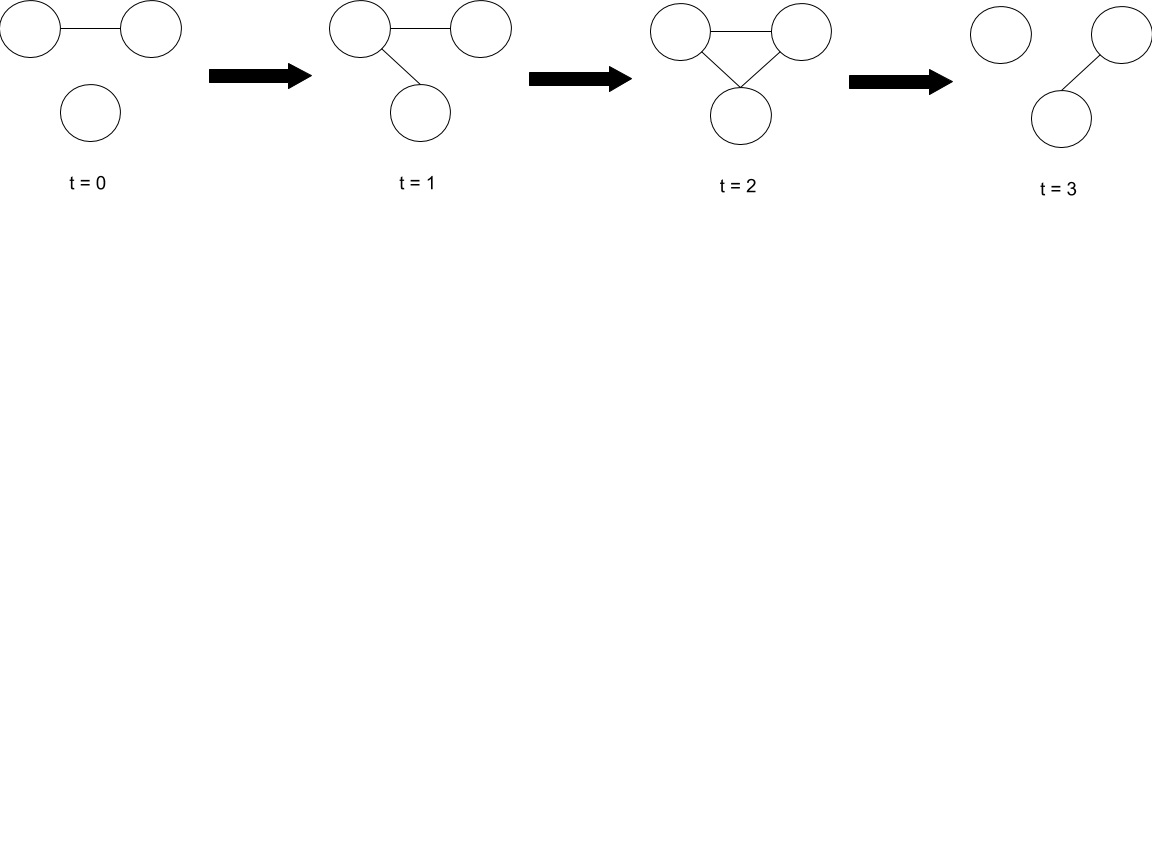
\includegraphics[trim={0 19cm 0 0}, clip, width=140mm]{./Figures/exampleDynamicNetwork.png}
\caption{An example of a dynamic network. The connections vary with time: a new connection is formed at t=1, another new connection is formed at t=2 and two are lost at t=3.}
\label{exampleDynamicNetwork}
\end{center}
\end{figure}

Naturally, dynamic networks are difficult to interpret and visualise quickly \cite{iddps}. Consider even a simple network composed of a handful of nodes and a handful of edges. Suppose we add the dynamic element to this simple network and mutate, say, the edges through a given time period. It can be difficult to interpret what, if anything those mutations indicate or represent even on a simple network. Many different approaches have been made to try and tackle this problem and mitigate the additional cognitive load. 

This report will focus on a novel approach - using a variety of easily interpretable \textit{measures} to produce some result based on either an aspect of the network at each frame of time or on the graph overall, for example: the density of the graph. Instead of manually stepping through the graph and attempting to pattern match, the measures can be observed. Using the measures to characterise the graph is somewhat conceptually similar to feature projection for dimensionality reduction \cite{wikidimred} in that the measures represent some feature vectors of the network and provide an abstract overview of the changes the network goes through, but since the measure visualisation is complementary to the existing network - rather than replacing it - the features aren't reduced but rather extracted and highlighted.
As more and more measures are added the resulting complexity requires that an intelligent visualisation of the measure values be implemented, since the goal is not to further add to the cognitive load but reduce it. Visualising these measures can allow us to spot patterns and trends over time, locate points of interest and motivate a hypothesis. Traditionally, network visualisations have been focused on visualising the changes themselves \cite{tsotaivg}, however here the measure-based approach aims to be more complementary to the network.

Although any type of network could have been used - care was taken while designing the measures and visualisations to keep them agnostic of the domain and avoid overfitting - a fairly small and simple social network was primarily used during development \ref{MARIEBOUCHER SOMEWHERE??}. 
%Social networks require less expert domain knowledge compared with say, biological networks to understand at a basic level [source or remove]. For the sake of simplicity I chose an easy to understand and rather small network. 
%Social networks are also more abstract than physical networks like power grids or computer networks \cite{taasodnv}.
Since this project aims to investigate dynamic network interpretation, using a simple network as a baseline ensures that difficulties in comprehension are not just inherent to the domain but to the network itself. 
%There are also a variety of existing networks that could be used to test against [source/example].
%Social network analysis provides a novel window by allowing the impacts to be quantified at the individual level, and the links between past, current and future behaviour to be carried across contexts. <https://besjournals.onlinelibrary.wiley.com/doi/pdf/10.1111/1365-2656.12764>

Networks can be constructed and interpreted in different ways. The measures used in this report are designed for a network composed of eternal nodes, unweighted edges and undirected edges, where an edge is a connection that happens instantaneously between two nodes, as in type (a) of Figure \ref{fig:edgeTypes}, and a nodepair exists between two nodes in a given period of time if any edge occurs between them in that period. 

\begin{center}
\begin{tabular}{cc}
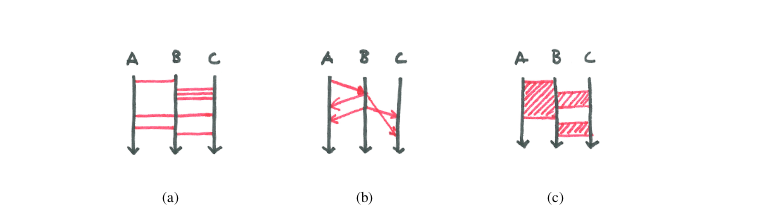
\includegraphics[trim={0 0 0 0}, width=140mm]{./Figures/edgeTypes.png}
\end{tabular}
\captionof{figure}{Types of connectivity. A, B and C represent nodes, time goes from top to
bottom, edges are indicated in red. (a) Instantaneous edges, (b) Transmissive edges, (c)
Persistent edges. \newline Figure and description taken from Connections, Changes and Cubes: Unfolding Dynamic Networks for Visual Exploration \cite{cccudnfve}.
}
\label{fig:edgeTypes}
\end{center}

Adjusting any of these assumptions would affect the selection of measures. Further work could be done on measures that take into account edge weight, persistent edges etc. The measures were also designed with social networks primarily in mind, but could of course be applied in other domains.

I extend the functionality of The Vistorian \cite{bach:hal-01205822} - an ongoing open source project by Bach et al. to create an online platform which provides interactive visualization for various kinds of networks, designed for social scientists and historians. 



%%Benjamin mentioned Objectives/Tasks section

\section{Contributions}
\label{objectives}
\begin{itemize}
    \item Summary of the literature regarding dynamic network visualisation.
    \item Development and evaluation of novel local dynamic measures - Local volatility, local activity and local redundancy.
    \item Development and evaluation of novel global dynamic measures - Global volatility, global activity and global redundancy.
    \item Extension of The Vistorian through:
    \begin{itemize}
        \item Creation of intuitive visualisations for local and global measures embedded into the existing interface.
        \item Implementing an extensible framework that ensures both new local and global measures can be easily visualised.
        \item Implementation of methods to calculate measures.
    \end{itemize}
    \item Demonstration of visualisations and measures in usage scenarios.

\section{Methodology}

To begin, I researched existing visualisation techniques for dynamic networks and various network measures. After selecting a few traditional measures I was able to implement basic prototype using those measures and a basic corresponding visualisation. I then iterated on both the visualisation and measures until the system was reasonably usable as a proof of concept. This provided a foundation to be able to add more experimental measures.

To obtain some external feedback on the progress I had made, an informal feedback meeting was held with with 4 active researchers on network analysis. These researchers were Dr Jim Lowe (James.Lowe@ed.ac.uk), Dr Miguel Garcia Sancho Sanchez (miguel.gsancho@ed.ac.uk), Mark Wong (Mark.Wong@glasgow.ac.uk) and Gil Viry (gil.viry@ed.ac.uk). I demonstrated usage of The Vistorian and the additions I had made for around 10 minutes, there was then around 15 minutes of discussion. In general there was a very positive reaction, which helped to validate the new additions and the following discussion inspired a new measure. The measures and visualisations were further iterated on, then more feedback was received from Pascal Cristofoli (pascal.cristofoli@ehess.fr). He experimented with the new additions and suggested two new measures be added as he often found himself calculating them manually. Implementing these two inspired a further two measures.  
\end{itemize}






%%%%%%%%%%%%%%%%%%%%%%%%%%%%%%%%%%%%%%%%%%%%%%%%%%%%%%%%%%%%%%%%%%%%%%%%%%%%%%%%
%2345678901234567890123456789012345678901234567890123456789012345678901234567890
%        1         2         3         4         5         6         7         8
% THESIS Chapter

\chapter{Background}

\section{Current Dynamic Network Visualisation Techniques}

In 2014 an investigation was done into the state of the art of visualising the dynamic element or third dimension \cite{tsotaivg}. Whilst this report will focus on using measure visualisations as a dynamic network visualisation technique it can be useful to see how the temporal element was directly visualised at a network level.

One such dynamic visualisation technique is using 'animations' or 'movies'. SoNIA \cite{sonia} for example is a node-link animation based dynamic network visualisation tool that aims "to handle network data and visualization in ways that explicitly deal with its time-based nature and aids the user in understanding what their data really mean" \cite{taasodnv}. SoNIA can be used to save the network animation as a quicktime movie. An interesting technique used in SoNIA is the interpolation of points between changes, to create smoother transitions that are more easily followed by the human eye. SoNIA has been successfully used for modelling interaction networks, disease transmission and football passing patterns demonstrating that animations are a feasible tool for visualising changes in network structure.

A common method of visualising static networks is the use of an adjacency matrix. Matrix Cubes \cite{vdnwmc} applies this technique to dynamic networks. Matrix cubes take the adjacency matrix of each static slice of a dynamic network and stacks them next to each other in order - using time as the third dimension, creating a cube. 
%Matrixes are more readable for larger and denser graphs with nodelink found to be worse than a matrix representation for static networks composed of over 20 nodes \cite{acotrogunlambr}.

When using a series of static node-link diagrams there are two methods to visualise the changes - one after the other (time-multiplexed) or side by side (juxtaposed) \cite{vdnwmc}. 


While The Vistorian's node-link diagram is timeline based the novel approach taken in this report is measure based and visualised alongside the existing timeline based approach. Since the local measures values are calculated based on the time window set in the timeline and the global measures use it directly as an axis, the measure based approach is tightly intertwined with the timeline approach. The measures themselves and their own accompanying visualisations are used to aid user's understanding of the networks changes - complementing the  timeline approach rather than replacing it.


\subsection{Measures}
A static measure, for example degree centrality, quantifies some aspect of a static network. They can be either local - based on a single node, or global - based on the network as a whole. Density is an example of a global static measure. 

Dynamic measures on the other hand fall into two categories. In the first category are measures which only make sense in a dynamic context and could not be applied to a strictly static network. In the second, static measures are applied and calculated at each time-frame, where a time-frame is the unit of change. %more?
Dynamic measures can also be described as local or global.



\section{Technologies}
\subsection{JavaScript and D3}
\label{sec:sec24}
The Vistorian was primarily written in TypeScript and D3 \cite{d3site}. Since I'm more comfortable working directly with Javascript all code was implemented using Javascript. D3 was used for the visualisations.

\subsection{Vistorian Implementation}

\begin{center}
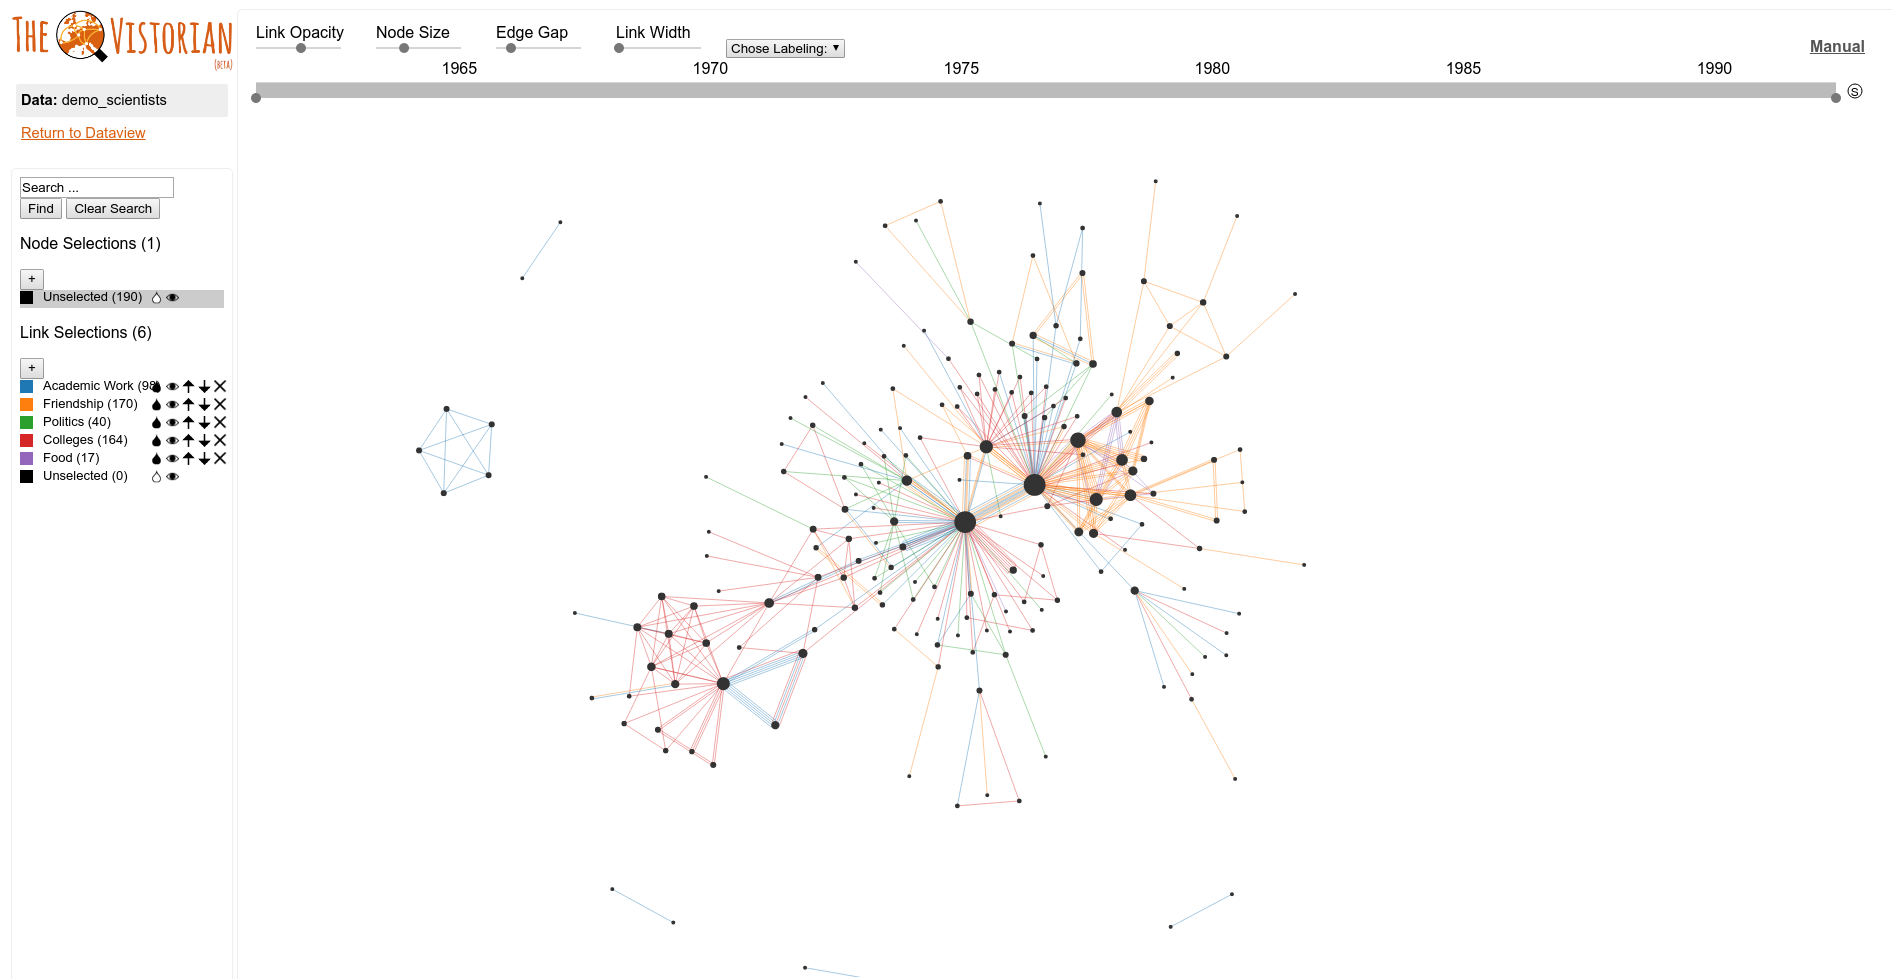
\includegraphics[trim={0 0 0 0}, width=140mm]{./Figures/vistorianOriginal.png}
\end{center}

More details are given in the visualization manual \cite{vismanual} but a summary of the key aspects is provided below.
This project will focus on the ‘Node-link’ visualisation specifically. The node-link diagram is composed of nodes as points and edges as straight lines. The positions of nodes are kept the same for all time-frames, making it easier to visualise \cite{tsotaivg}. It's also simple and intuitive.
%-Node-link history and development, why I'm using this one.\newline <-?
At the top of the network page is a time-slider. Adjusting this time slider filters the links shown if they are not present in that window. A force-directed layout is used, meaning that nodes with many common neighbours are drawn close to each other and nodes with fewer connections are moved to the edges. Node size is used to indicate the node degree and line colour indicates a specific type of relation. Edges are defined as the direct links between nodes and only exist during at most one time-frame, whereas a nodepair is active if any edge is present between two nodes - meaning they can exist during multiple time-frames provided there is at least one edge linking the nodes. In The Vistorian the network is split into discrete time-frames where each time-frame represents some change happening in the network. 






%%%%%%%%%%%%%%%%%%%%%%%%%%%%%%%%%%%%%%%%%%%%%%%%%%%%%%%%%%%%%%%%%%%%%%%%%%%%%%%%
%2345678901234567890123456789012345678901234567890123456789012345678901234567890
%        1         2         3         4         5         6         7         8
% THESIS CHAPTER

\chapter{Work Undertaken}

% short summary of the chapter
\section*{Measures}

\section{Final User Interface}
Figure X contains the final user facing implementation. 
\begin{center}
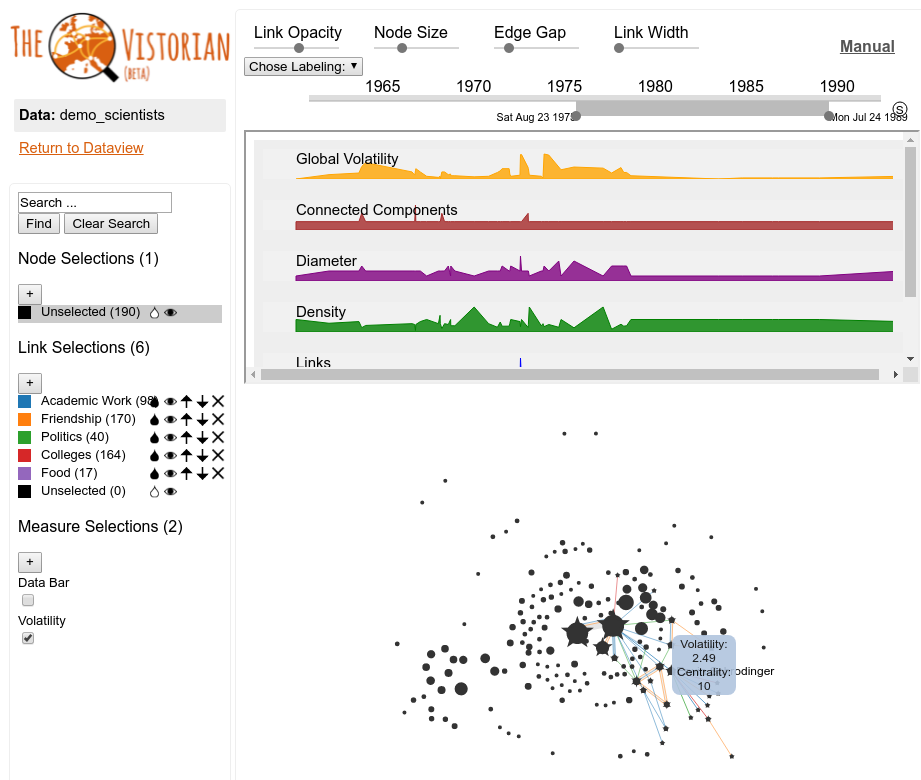
\includegraphics[trim={0 0 0 0}, width=140mm]{./Figures/finalUI.png}
\end{center}

\subsection{The Databar}

\begin{center}
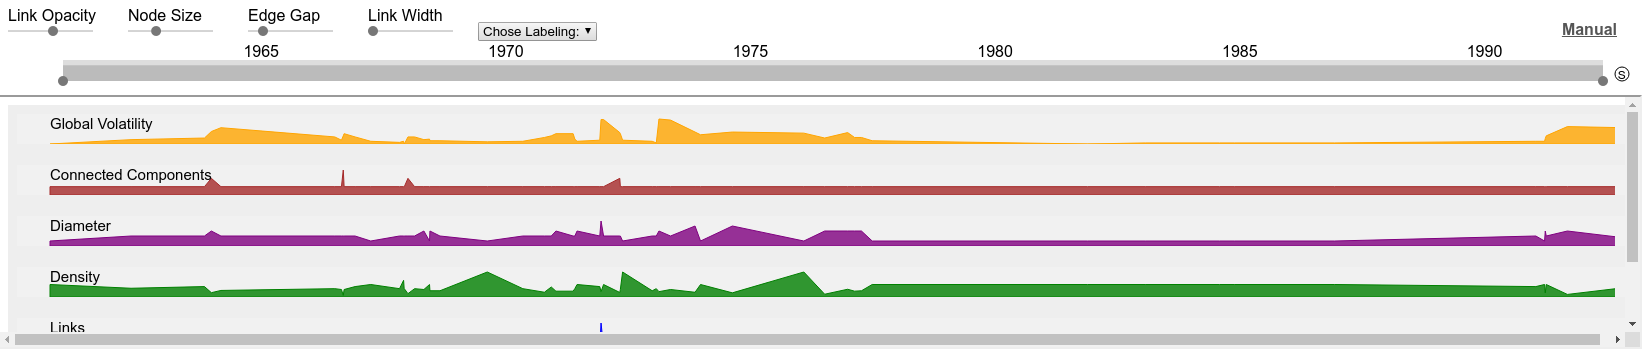
\includegraphics[trim={0 0 0 0}, width=140mm]{./Figures/databar.png}
\end{center}

The Databar holds the visualisation graphs for global measures. I decided to place it along the top of the window because it would line up nicely with the pre-existing timeline which could then double as the x-axis label - saving valuable screen space.
The databar is highly interactive. Each graph is initially collapsed and can then be expanded by clicking. As more measures were added I realised that it wouldn't be possible to both provide enough detail in every graph and also facilitate easy comparison without taking up most of the screen real estate. Collapsing and expanding the graphs solved this problem. The databar was designed to be readily extensible and only needs to be provided with a list of values the same length as the number of time-frames. It then maps each value to the corresponding time frame to produce the co-ordinate values for the ridgeline. 

\begin{center}
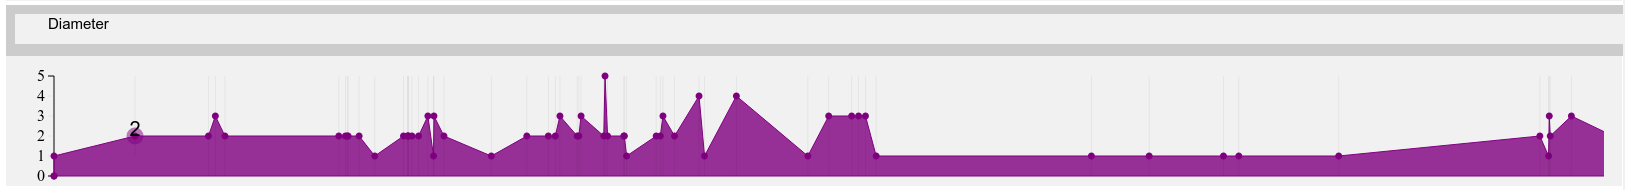
\includegraphics[trim={0 0 0 0}, width=140mm]{./Figures/diameterGraph.png}
\end{center}
A d3 scale is used to provide the y axis labels seen on the left of the expanded graph. Moving the mouse across the screen causes a cursor to track along the ridgeline of the graph. The y-label at that point is shown on the tracker. This was originally done when the graphs weren't expandable to remove the need for an axis and save space, however it was found to be useful for tightly clumped values and for data with some small step sizes.
\begin{center}
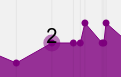
\includegraphics[trim={0 0 0 0}, width=35mm]{./Figures/ridgeTracker.png}
\end{center}
The vertical lines indicate a timestep/change in the graph. This was orignally simply intended to make it easier for the user to  compare graphs vertically, however an additional and powerful benefit is that it allows the user to  easily finding time periods of high or low activity.
Finally, graphs can be reordered for easy comparison using click and drag as there is not enough screen space to see all graphs at once, even compressed.

\section{Measures and Visualisations}
The measures that have been implemented are each detailed below. The methods of calculation, the reasons for selecting them, their applications in The Vistorian and potential further applications are provided.

%%%%%%%%%%%%%%%%%%%%%%%%%%%%%%%%%%%%%%%%%%%%%%%%%%%%%%%%%%%%%%%%%%%%%%%%%%%%%%%%%%%%%%%%%%%%%%%%%%%%%%%%%%%%%%%
%NUMBER OF Nodepairs
%%%%%%%%%%%%%%%%%%%%%%%%%%%%%%%%%%%%%%%%%%%%%%%%%%%%%%%%%%%%%%%%%%%%%%%%%%%%%%%%%%%%%%%%%%%%%%%%%%%%%%%%%%%%%%%
\subsection{Number of Nodepairs}
%\subsubsection{Summary}
Simply the total number of active nodepairs in the network at a given time - a global static measure quantified at each time-frame. It gives a quick idea of the degree of activity during a time frame.

%\subsubsection{Reasons for Selection}
The number of nodepairs is one of the most basic measures. However it aids understanding of the network considerably as it provides perhaps the simplest way of understanding the overall size of the network at a time-frame or how it varies during a period, keeping cognitive load low while still improving understanding considerably.

%\subsubsection{Vistorian Implementation}
In The Vistorian this measure is interpreted as the number of connections at each time-frame, so this measure shows how that number changes over time.
%\subsubsection{Visualisation}                                                                                
%\subsubsection{Further Applications}


%%%%%%%%%%%%%%%%%%%%%%%%%%%%%%%%%%%%%%%%%%%%%%%%%%%%%%%%%%%%%%%%%%%%%%%%%%%%%%%%%%%%%%%%%%%%%%%%%%%%%%%%%%%%%%%
%NUMBER OF ACTIVE NODES
%%%%%%%%%%%%%%%%%%%%%%%%%%%%%%%%%%%%%%%%%%%%%%%%%%%%%%%%%%%%%%%%%%%%%%%%%%%%%%%%%%%%%%%%%%%%%%%%%%%%%%%%%%%%%%%
\subsection{Number of Active Nodes}
%\subsubsection{Summary}
Another global static measure. The number of active nodes is calculated as the total number of nodes with at least one edge in the network for each timeframe.

%\subsubsection{Reasons for Selection}
Like the number of edges, the number of active nodes is also a very basic measure. However it gives an easily interpretable sense of the number of actors at a given time. Knowing if activity is high because there are multiple actors or because those actors are each very active is important to be able to distinguish. As it is a simple measure it also keeps cognitive load low while still improving understanding considerably.

%\subsubsection{Vistorian Implementation}
In the Vistorian this gives an idea of the number of people involved at each time frame, either sending or receiving messages. 

%\subsubsection{Visualisation}
%\subsubsection{Further Applications}

%%%%%%%%%%%%%%%%%%%%%%%%%%%%%%%%%%%%%%%%%%%%%%%%%%%%%%%%%%%%%%%%%%%%%%%%%%%%%%%%%%%%%%%%%%%%%%%%%%%%%%%%%%%%%%%
%DIAMETER
%%%%%%%%%%%%%%%%%%%%%%%%%%%%%%%%%%%%%%%%%%%%%%%%%%%%%%%%%%%%%%%%%%%%%%%%%%%%%%%%%%%%%%%%%%%%%%%%%%%%%%%%%%%%%%%
\subsection{Diameter}
%\subsubsection{Summary}
The longest of all shortest paths in the network at a given time. Diameter gives a sense of the interconnectedness of a network. A high diameter would mean the network is quite loose and linear, a low diameter implies nodes tend to be tightly connected with each other - however there could of course be a particularly long branch responsible for creating a high value. Diameter is applied as a global static measure.

%\subsubsection{Reasons for Selection}
Diameter was selected as a measure because no other measure gives a sense of network breadth. It works particularly well alongside density to paint a picture of how the shape of the network evolves over time.
%Diameter is particularly important in social networks. The commonly known six-degrees of separation theory https://www.jstor.org/stable/pdf/2786545.pdf?acceptTC=true effectively states that if one were to make a social networks of all humans, the expected diameter would be 6. In a dynamic context... 

%\subsubsection{Vistorian Implementation}
In The Vistorian the diameter gives a sense of social distance or degrees of separation between individuals in a ‘conversation’. <may need defined> 
%\subsubsection{Visualisation}
%\subsubsection{Further Applications}

%%%%%%%%%%%%%%%%%%%%%%%%%%%%%%%%%%%%%%%%%%%%%%%%%%%%%%%%%%%%%%%%%%%%%%%%%%%%%%%%%%%%%%%%%%%%%%%%%%%%%%%%%%%%%%%
%DENSITY
%%%%%%%%%%%%%%%%%%%%%%%%%%%%%%%%%%%%%%%%%%%%%%%%%%%%%%%%%%%%%%%%%%%%%%%%%%%%%%%%%%%%%%%%%%%%%%%%%%%%%%%%%%%%%%%
\subsection{Density}
%\subsubsection{Summary}
Density here is defined as (THIS FORMULA). It gives a sense of connectedness at a given period of time. Only nodes with at least one edge are counted. Essentially, if every node is connected to every other node then density will be 1. Density is a global static measure.

%\subsubsection{Reasons for Selection}
Density is used as one of the measures because it gives the user an overview of how interconnected the graph is at a given point and how that varies over time. Since the goal is to provide as much information about the behaviour of the graph as possible using as few measures as possible it is important that information overlap from different measures is minimised. An overview of density can't be easily gathered from observing the graph and it can't be easily extrapolated from the other selected methods.

%\subsubsection{Vistorian Implementation}
We define an active node as node that has sent or received a letter during a time frame. In The Vistorian a density of 1 at a time frame means that every active node during that time frame has either sent or received a letter from every other active node.

%\subsubsection{Visualisation}

%\subsubsection{Further Applications}

%%%%%%%%%%%%%%%%%%%%%%%%%%%%%%%%%%%%%%%%%%%%%%%%%%%%%%%%%%%%%%%%%%%%%%%%%%%%%%%%%%%%%%%%%%%%%%%%%%%%%%%%%%%%%%%
%NUMBER OF CONNECTED COMPONENTS
%%%%%%%%%%%%%%%%%%%%%%%%%%%%%%%%%%%%%%%%%%%%%%%%%%%%%%%%%%%%%%%%%%%%%%%%%%%%%%%%%%%%%%%%%%%%%%%%%%%%%%%%%%%%%%%
\subsection{Number of connected components}
\subsubsection{Summary}
A connected component is a full group of nodes connected by edges. This measure is simply the number of discrete connected components. It is a global static measure.
Figure below has two connected components.

\begin{center}
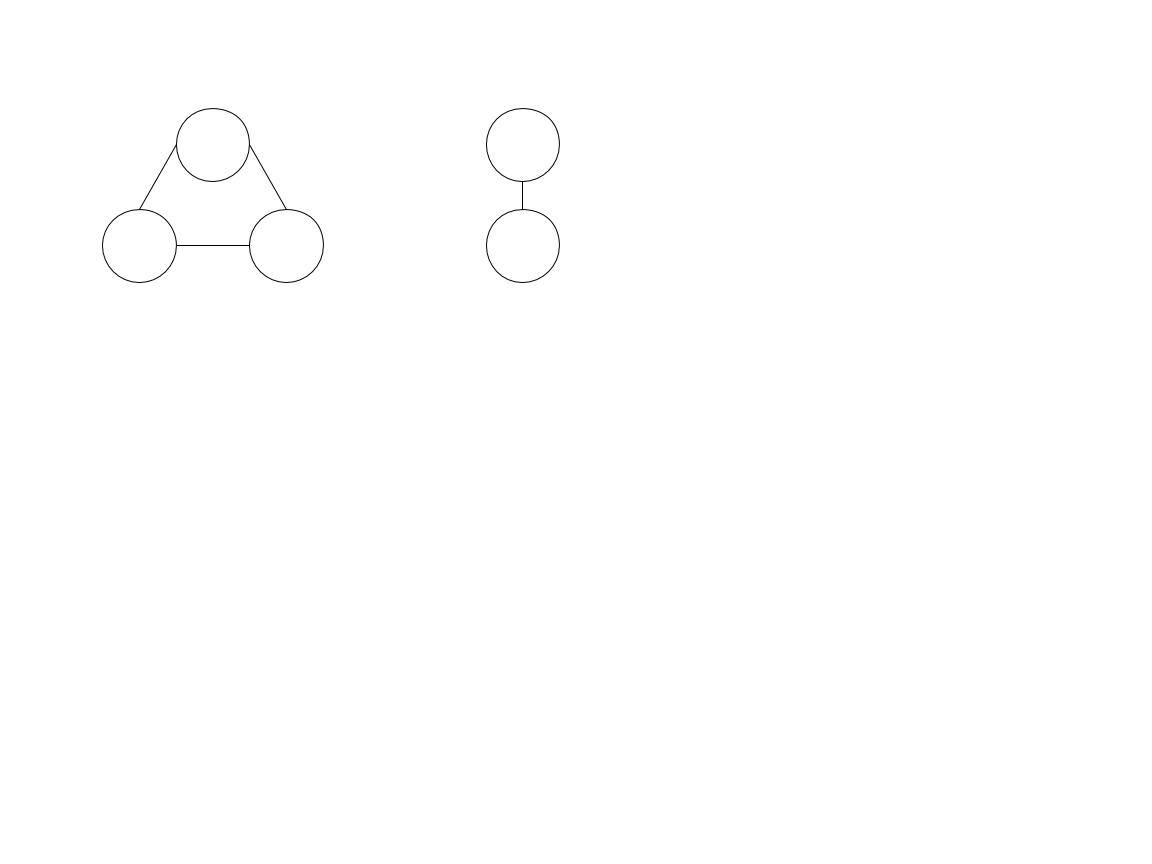
\includegraphics[trim={0cm, 20cm, -10cm, 0cm}, width=180mm]{./Figures/connectedComponents1.jpg}
\end{center}

%\subsubsection{Reasons for Selection}
The number of connected components was selected as a measure because it shows how many distinct groups there are at any given point. The user could then step through the graph to see how these groups evolve over time.

%\subsubsection{Vistorian Implementation}
In The Vistorian, this measure can be interpreted as the number of distinct conversations happening during a given chunk of time. 

%\subsubsection{Visualisation}
%\subsubsection{Further Applications}

%%%%%%%%%%%%%%%%%%%%%%%%%%%%%%%%%%%%%%%%%%%%%%%%%%%%%%%%%%%%%%%%%%%%%%%%%%%%%%%%%%%%%%%%%%%%%%%%%%%%%%%%%%%%%%%
%CENTRALITY
%%%%%%%%%%%%%%%%%%%%%%%%%%%%%%%%%%%%%%%%%%%%%%%%%%%%%%%%%%%%%%%%%%%%%%%%%%%%%%%%%%%%%%%%%%%%%%%%%%%%%%%%%%%%%%%
\subsection{Centrality}
%\subsubsection{Summary}
Centrality here is a local measure. The specific implementation used is degree centrality [source]. Degree centrality is simply the number of edges connected to a node in the given time period. It can be interpreted as static here despite being applied to a time-period rather than a time-frame because it effectively treats that time-period as a fixed frame.

%\subsubsection{Reasons for Selection}
Degree centrality was implemented concretely in the project to complement the pre-existing visualisation - the size of nodes in the nodelink diagram in The Vistorian is fixed and proportional to the number of connected edges they have during the full time window. However since this changes for each time-frame it's convenient to be able to read off the exact value, particularly for highly connected nodes with many links.

%\subsubsection{Vistorian Implementation}

%\subsubsection{Visualisation}
%\subsubsection{Further Applications}


%%%%%%%%%%%%%%%%%%%%%%%%%%%%%%%%%%%%%%%%%%%%%%%%%%%%%%%%%%%%%%%%%%%%%%%%%%%%%%%%%%%%%%%%%%%%%%%%%%%%%%%%%%%%%%%
%LOCAL VOLATILITY
%%%%%%%%%%%%%%%%%%%%%%%%%%%%%%%%%%%%%%%%%%%%%%%%%%%%%%%%%%%%%%%%%%%%%%%%%%%%%%%%%%%%%%%%%%%%%%%%%%%%%%%%%%%%%%%

\subsection{Local Volatility}

\subsubsection{Development}

NEW THOUGHTS TO ADD
- Order doesn't matter.
- Each std will be between 0 and 0.5 due to the binary values.
- 

In my literature review I didn’t come across any examples where this specific measure, or anything similar, was used or investigated. I felt that there needed to be some measure or score which captured the level of connection fluctuation such that a node whose connections tended to stay mostly within a fixed set of other nodes would score low but a node whose edges tended to be short lived and with unfamiliar nodes would score high. This was a highly experimental process as there are a number of ways this could be achieved.
Volatility is a local measure, calculate for a node and with respect to a set start time and end time. Initially it was calculated as the population standard deviation of the number of a node’s connections throughout that time period, effectively the variance in the number of connections.

\begin{center}
$N = total\ number\ of\ time\ frames$
$\overline{x} = average\ number\ of\ connections\ from\ given\ node $
$x_i = number\ of\ connections\ at\ time\ i$

$local\ volatility\ = \sqrt{\frac{1}{N} \sum_{i=1}^N (x_i - \overline{x})^2}$
\end{center}

Examples are given below, calculated for the central node.


\begin{center}
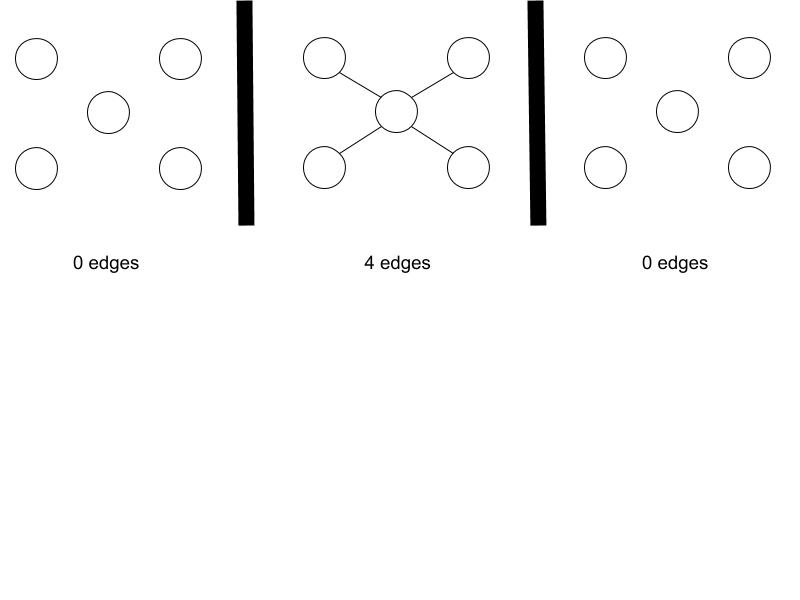
\includegraphics[trim={0 10cm 0 -1cm}, width=120mm]{./Figures/volatility1.jpg}

$N = 3$

$\overline{x} = \frac{4 + 0 + 0}{3} = \frac{4}{3}$

$local volatility =\frac{1}{3}\times((0 - \frac{4}{3})^2 + ((4 - \frac{4}{3})^2) + (0 - \frac{4}{3})^2) $

$local volatility = 1.89$

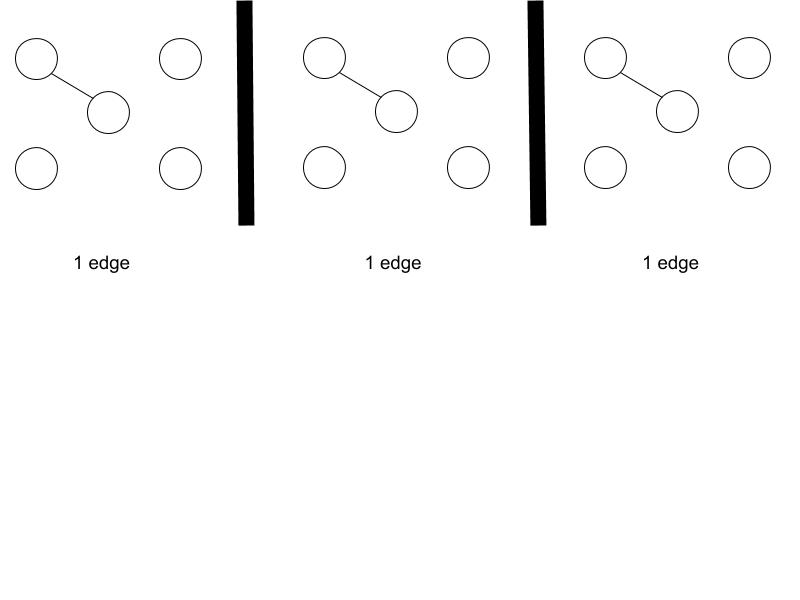
\includegraphics[trim={0 10cm 0 -1cm}, width=120mm]{./Figures/volatility2.jpg}

$N = 3$

$\overline{x} = \frac{1 + 1 + 1}{3} = 1$

$local volatility =\frac{1}{3}((1 - 1)^2 + ((1 - 1)^2) + (1 - 1)^2) $

$local volatility = 0$
\end{center}

Looking soley at these two examples this approach appears to work quite well - changes in edges results in a higher local volatility whereas no changes results in 0 local volatility.

However the problem with this approach is that it maintains no ‘memory’ of which edges were previously connected, consider the example below.
\begin{center}
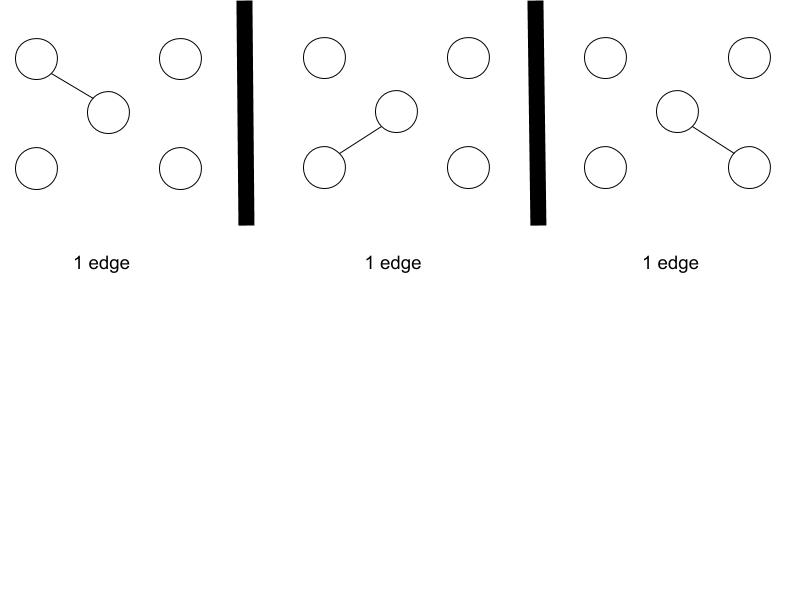
\includegraphics[trim={0 10cm 0 -1cm}, width=120mm]{./Figures/volatility3.jpg}
\end{center}

The local volatility will still be 0 despite the edge changing since only the number of edges is taken into account.

To fix this we must have some way to track individual edges, rather than solely the quantity. A solution is to give edges unique ids and store a binary value tracking which edges are present at each time frame and then sum the standard deviations of these. Example below, again calculated for the central node.

\begin{center}
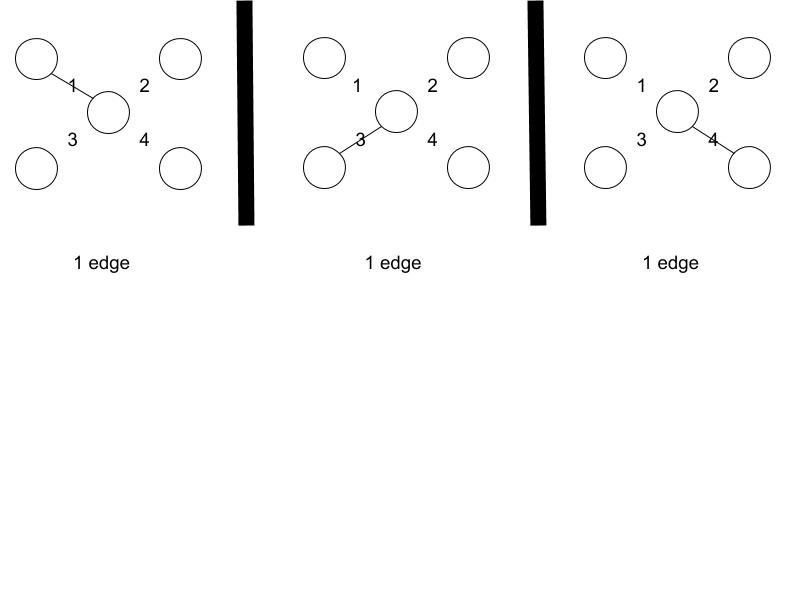
\includegraphics[trim={0 10cm 0 -1cm}, width=120mm]{./Figures/volatility4.jpg}
\end{center}

We store an object mapping as follows:

$edge_id: [binary\ value\ indicating\ presence\ during\ timestep\ at\ index].$

\begin{center}
\{1:[1, 0, 0], 3: [0, 1, 0], 4: [0, 0, 1]\}
\end{center}
Local volatility could then be calculated as the average of the standard deviations of the object values.
\begin{center}
$local\ volatility = \frac{std([1,0,0]) + std([0,1,0]) + std([0,0,1])}{3}$

$local\ volatility = 0.47$
\end{center}

This approach too has an initially subtle problem however. Consider the figures below.
\begin{center}
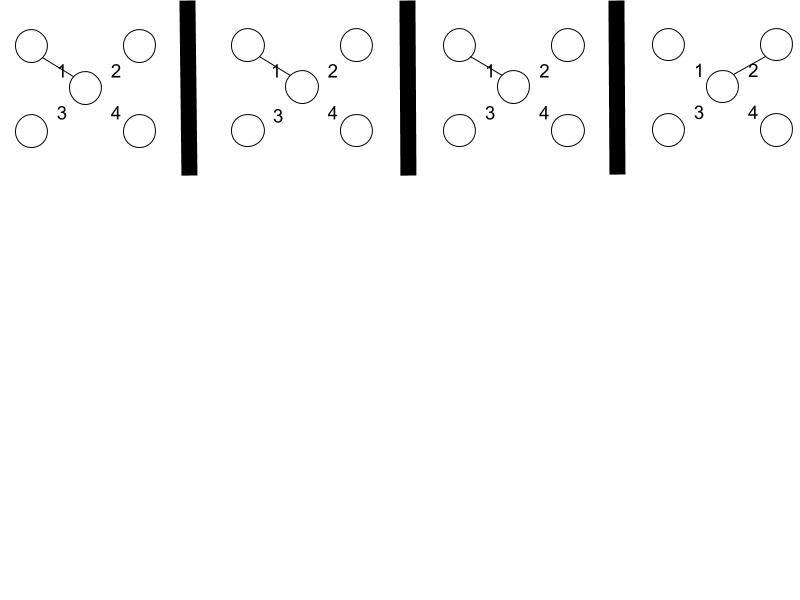
\includegraphics[trim={0 10cm 0 -1cm}, width=120mm]{./Figures/volatilityLastProblem1.jpg}
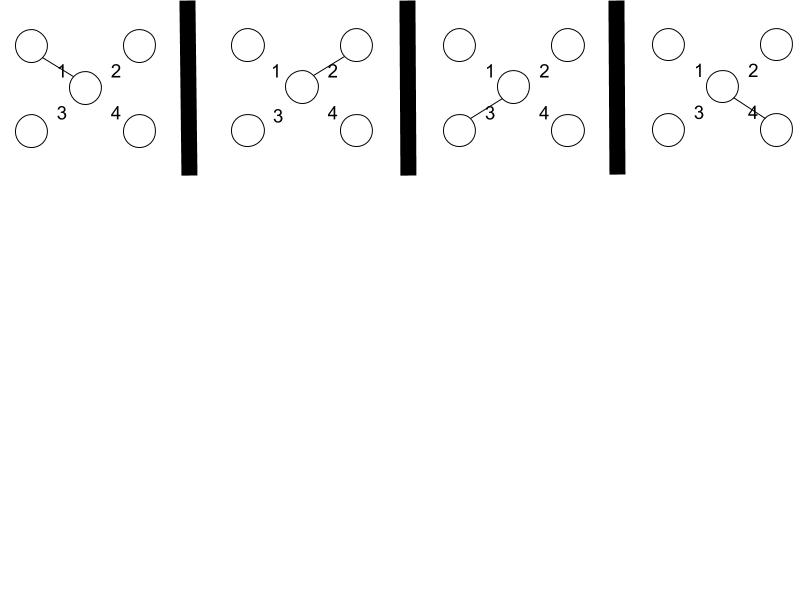
\includegraphics[trim={0 10cm 0 -1cm}, width=120mm]{./Figures/volatilityLastProblem2.jpg}
\end{center}
The volatility for the central node of the first network here would be calculated as follows.

\begin{center}
$N = 2$

$Mapping = \{1:[1, 1, 1, 0], 2:[0, 0, 0, 1]\}$

$local\ volatility = \frac{std([1,1,1,0]) + std([0,0,0,1])}{2}$

$local\ volatility = 0.43$
\end{center}

However upon calculating the volatility for the central node of the second network we find that it is equal. This is a problem because on observing the networks it can be seen that in network 1 there is a relatively stable edge, 1, for three of four time steps. Network 2 however has no edge lasting more than one time frame. This result does not align with the given specification of volatility, the second network should have a lower value than the first.

\begin{center}
$N = 4$

$Mapping = \{1:[1, 0, 0, 0], 2:[0, 1, 0, 0], 3: [0, 0, 1, 0], 4: [0, 0, 0, 1]\}$

$local\ volatility = \frac{std([1,0,0,0]) + std([0,1,0,0]) + std([0,0,1,0]) + std([0,0,0,1])}{4}$

$local\ volatility = 0.43$
\end{center}

The problem is caused by the averaging and the fact that the order of items does not affect standard deviation. My solution to this problem was to outright remove the averaging, and simply sum the terms. Since this could quickly lead to some very high values a log-scale is used for the visualisation. More details are provided on this in the visualisation method section\link{BLANK}.  

With this fix the local volatility for the central node of the first network is 1.73 and 0.86 for the second network. 

To summarise, local volatility is calculated on a node. It is calculated as the cumulative sum of the standard deviations of the binary presences of each node that is present at least once in the given time frame.

Several more examples were worked through to ensure that volatility behaved as a user would expect given the way it is described. [SHOW THESE IN AN APPENDIX??]

Since responsiveness is key, some space complexity is sacrificed. A large data structure is initialised on page load mapping nodes to nodepairs and nodepairs to their binary presence values at each timeframe.
I considered further optimising by only storing positive presence values and extrapolating the negatives as needed for the standard deviation calculations, however this additional calculation would reduce responsiveness which is already somewhat limited in the browser.

\subsubsection{Vistorian Implementation}
Whilst this solution would work well in a general case it works poorly in The Vistorian as edges only appear once. To fix this we instead use node-pairs. 
Local volatility in The Vistorian gives a sense of the variation of a node's social contacts in a given time period. This is useful in the Vistorian because it allows us to see if one contact was rapidly sending or receiving messages to or from new contacts, or if they maintained fairly constant communication with a select number. 


\subsubsection{Further Applications}
Local volatility could have broad applications in other domains where dynamic networks are used. 
\newline\newline
Say a system administrator was conducting a post-mortem of an attack on a network using a dynamic network analysis tool to determine which nodes were potentially behaving maliciously. One measure useful in determining an anomaly in a network is the number of successfully established TCP connections in a time interval \cite{fnpfid}. A malicious port scan usually sends a relatively small number of packets to a large number of hosts on a network \cite{fnpfid}. If a similar volatility measure was implemented in this dynamic network analysis tool and TCP connections were considered to be edges it would be very easy for the system administrator to spot particularly volatile, or spiky, nodes.
\newline\newline
Whilst investigating different proteins in protein-protein interaction networks and their impact on the development and progression of hepatocellular carcinoma (HCC) after hepatitis C virus infection the protein core ESR1, which interacted with most of the nodes in the randomly selected sub-network, was shown to be associated with an increased HCC risk \cite{acaotdbnihih}. Using local volatility as a measure while performing this anaylsis would have immediately highlighted the ESR1 protein as highly volatile and worthy of further investigation.

%%%%%%%%%%%%%%%%%%%%%%%%%%%%%%%%%%%%%%%%%%%%%%%%%%%%%%%%%%%%%%%%%%%%%%%%%%%%%%%%%%%%%%%%%%%%%%%%%%%%%%%%%%%%%%%
%GLOBAL VOLATILITY
%%%%%%%%%%%%%%%%%%%%%%%%%%%%%%%%%%%%%%%%%%%%%%%%%%%%%%%%%%%%%%%%%%%%%%%%%%%%%%%%%%%%%%%%%%%%%%%%%%%%%%%%%%%%%%%

\subsection{Global Volatility}

%\subsubsection{Development}
To obtain some external feedback on the progress I had made an informal feedback meeting was held with with 4 active researchers on network analysis. These researchers were Dr Jim Lowe (James.Lowe@ed.ac.uk), Dr Miguel Garcia Sancho Sanchez (miguel.gsancho@ed.ac.uk), Mark Wong (Mark.Wong@glasgow.ac.uk) and Gil Viry (gil.viry@ed.ac.uk). I demonstrated usage of The Vistorian and the additions I had made for around 10 minutes, there was then around 15 minutes of discussion. In general there was a very positive reaction, which helped to validate the new additions. It was mentioned that a sense of overall volatility could be useful to complement the local volatility measure. This could be used to investigate if a node's local volatility was high simply because overall volatility was high or if it is worthy of further investigation. This became Global Volatility.

Global volatility is similar to local volatility in that it is a measure of change. It is defined as the change in active nodepairs for each time-frame, starting from 0. If a nodepair wasn't active in the previous time-frame but is active in the next then global volatility will be increased by one. Similarly if a nodepair was active in the previous time-frame but wasn't active in the next then global volatility would also be increased by one as this is also a change. In figure X the values at each timestep would be [0, 2, 2].

\begin{center}
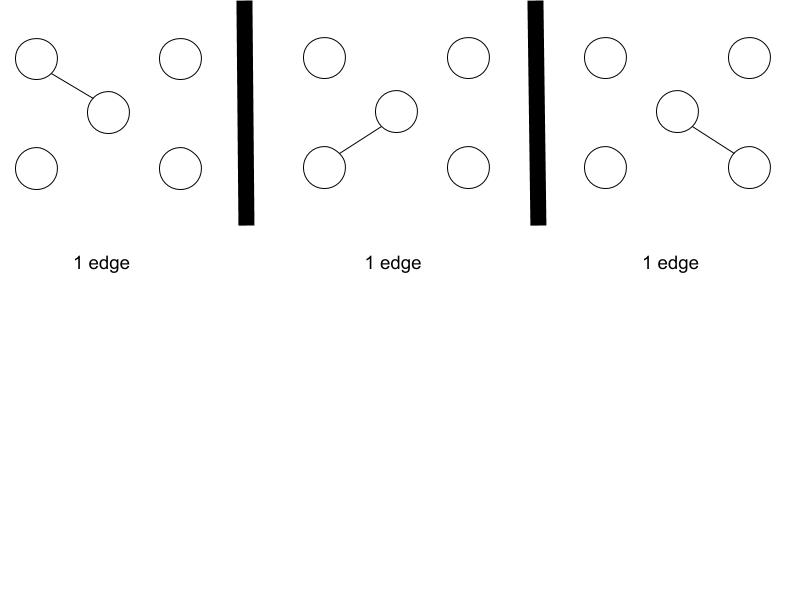
\includegraphics[trim={0 10cm 0 -1cm}, width=120mm]{./Figures/volatility3.jpg}
\end{center}



%\subsubsection{Vistorian Implementation}

%\subsubsection{Visualisation Method}

%\subsubsection{Further Applications}


%%%%%%%%%%%%%%%%%%%%%%%%%%%%%%%%%%%%%%%%%%%%%%%%%%%%%%%%%%%%%%%%%%%%%%%%%%%%%%%%%%%%%%%%%%%%%%%%%%%%%%%%%%%%%%%
%GLOBAL ACTIVATION
%%%%%%%%%%%%%%%%%%%%%%%%%%%%%%%%%%%%%%%%%%%%%%%%%%%%%%%%%%%%%%%%%%%%%%%%%%%%%%%%%%%%%%%%%%%%%%%%%%%%%%%%%%%%%%%

\subsection{Global Activation}
Global activation is a global dynamic measure. It is defined at each frame as the cumulative count of the number of new nodes that have been added, meaning that it will begin at 0 in the first frame, and end as the total number of nodes at the last frame. Observing this measure gives a sense of the rate at which new nodes are added. 

In The Vistorian, if global activation rapidly peaked and then only slowly climbed to the maximum but we also knew that activity was fairly constant this would imply that few new actors are added throughout the period and that most of the activity is between actors that have sent or received messages before.

In figure X above global activation would be [1, 2, 3].

%\subsubsection{Development}


%%%%%%%%%%%%%%%%%%%%%%%%%%%%%%%%%%%%%%%%%%%%%%%%%%%%%%%%%%%%%%%%%%%%%%%%%%%%%%%%%%%%%%%%%%%%%%%%%%%%%%%%%%%%%%%
%GLOBAL REDUNDANCY
%%%%%%%%%%%%%%%%%%%%%%%%%%%%%%%%%%%%%%%%%%%%%%%%%%%%%%%%%%%%%%%%%%%%%%%%%%%%%%%%%%%%%%%%%%%%%%%%%%%%%%%%%%%%%%%

\subsection{Global Redundancy}
Global redundancy is a global dynamic measure and is linked with global activation. It is defined as the number of nodes at each time frame that have been active in any previous time frame. Observing this measure gives a sense of the number of repeated nodes. A low redundancy implies that most nodes are only fairly inactive. A high redundancy implies that nodes are more active and reconnect often.

In figure X above global redundancy would be [0, 0, 0].


%\subsubsection{Development}


%%%%%%%%%%%%%%%%%%%%%%%%%%%%%%%%%%%%%%%%%%%%%%%%%%%%%%%%%%%%%%%%%%%%%%%%%%%%%%%%%%%%%%%%%%%%%%%%%%%%%%%%%%%%%%%
%LOCAL ACTIVATION
%%%%%%%%%%%%%%%%%%%%%%%%%%%%%%%%%%%%%%%%%%%%%%%%%%%%%%%%%%%%%%%%%%%%%%%%%%%%%%%%%%%%%%%%%%%%%%%%%%%%%%%%%%%%%%%

\subsection{Local Activation}

Pascal Cristofoli (pascal.cristofoli@ehess.fr) [...]. Experimented with the new additions. He suggested two new measures be added as he often found himself calculating them manually. These measures are local activation and local redundancy.

Local Activation is a local dynamic measure. It is calculated as the number of connections in the selected time period that weren't ever active before that time period began. In the network below\ref{} if the four time frames represent the full time period, the local activation value for the central node would be 3. If the selected time period was from the second to final time frames, inclusive, then the activation value for the central node would be 2.
\begin{center}
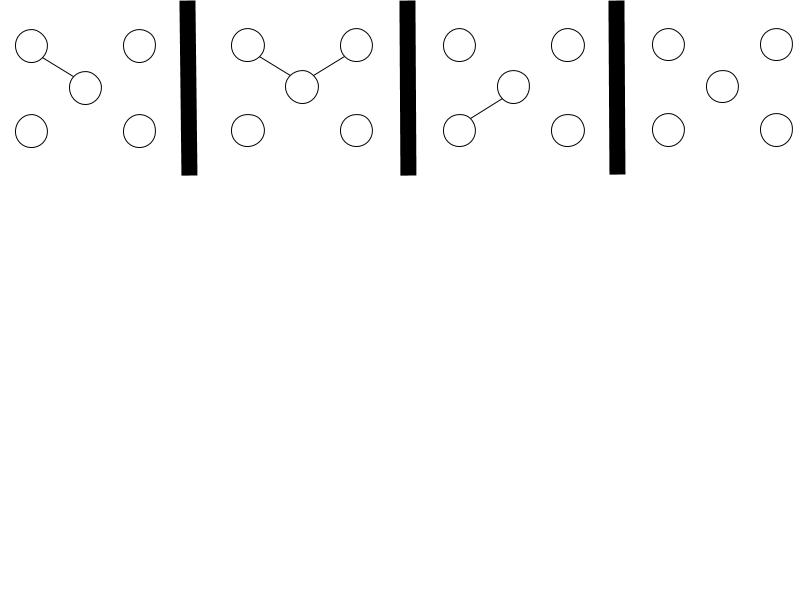
\includegraphics[trim={0 10cm 0 -1cm}, width=120mm]{./Figures/localActivation1.jpg}
\end{center}

\subsubsection{Further Applications}
Local activation could have broad applications in other domains where dynamic networks are used. 
\newline\newline


%%%%%%%%%%%%%%%%%%%%%%%%%%%%%%%%%%%%%%%%%%%%%%%%%%%%%%%%%%%%%%%%%%%%%%%%%%%%%%%%%%%%%%%%%%%%%%%%%%%%%%%%%%%%%%%
%LOCAL REDUNDANCY
%%%%%%%%%%%%%%%%%%%%%%%%%%%%%%%%%%%%%%%%%%%%%%%%%%%%%%%%%%%%%%%%%%%%%%%%%%%%%%%%%%%%%%%%%%%%%%%%%%%%%%%%%%%%%%%

\subsection{Local Redundancy}

Local Redundancy is also a local dynamic measure, highly complementary to local activation. It is calculated as the number of connections in the selected time period that have been active before that time period began. In the network figure above\ref{} if the four time frames represent the full time period, the local redundancy value for the central node would be 0, since there are no prior connections. If the selected time period was from the second to final time frames, inclusive, then the redundancy value for the central node would be 1.

\subsubsection{Further Applications}
Local activation could have broad applications in other domains where dynamic networks are used. 
\newline\newline
In 2002 a study was conducted using a network of business connections to investigate if the degree of redundancy in social networks influenced the success of business start-ups \cite{socRed}. Redundancy here is applied in a static sense, such that "In non‐redundant networks the entrepreneurs’ contacts do not know each other and rarely have the same information". If a dynamic network was used instead, and the local redundancy measure was applied then .... STATIC V DYNAMIC A BIT DIFFICULT HERE BUT I THINK IT COULD BE A GOOD ADDITION?

%%%%%%%%%%%%%%%%%%%%%%%%%%%%%%%%%%%%%%%%%%%%%%%%%%%%%%%%%%%%%%%%%%%%%%%%%%%%%%%%%%%%%%%%%%%%%%%%%%%%%%%%%%%%%%%
%LOCAL MEASURE VISUALISATION.
%%%%%%%%%%%%%%%%%%%%%%%%%%%%%%%%%%%%%%%%%%%%%%%%%%%%%%%%%%%%%%%%%%%%%%%%%%%%%%%%%%%%%%%%%%%%%%%%%%%%%%%%%%%%%%%
\section{Local Measure Hoverover}
To save screen space and reduce visual complexity, the precise values of a node's local measures given the selected time period are only shown on hover over. For the purposes of this report, the local measures are degree centrality and local volatility. However the implementation is easily extensible, allowing for more local measures to be quickly visualised.

Initially, local volatility was visualised using 'spikes', where more spikes indicated higher local volatility. Other methods were considered, vibration matches with the mental image of volatility but would be too distracting to the eye. Dotted rings with larger diameter indicating higher local volatility were considered but had too much potential for confusing overlap. Colours were originally used but could be misconstrued as relating to the edge colours. 
However as more local measures were added the spikes made less sense. They were also somewhat difficult to count on smaller nodes.

Local activation, redundancy, volatility and centrality are all visualised in the same way - as the radius of the node in the network visualisation. A drop down is used in the bookmarks bar [make sure this is shown on a labelled diagram at start] to select between them. The values are calculated for each node and the nodes radius is then calculated as the log of double the measures value, plus one. The values are doubled to give more visual separation which is hampered by the log scale. The "+1" is added so that nodes always have a radius to avoid breaking the user's mental map \cite{BLANK}.

To aid the user further, a lighter grey circle of a fixed radius is shown behind each node. It's radius is calculated given the active local measure as that measures value over the full time frame. This allows users to see how a smaller window of time differs from the full time period. It was considered to use the maximum value that the selected measure ever takes for each given node, however this would require considerable initial computation as all pairs of start and end times would have to be considered for every single node.

[pictures]


%%%%%%%%%%%%%%%%%%%%%%%%%%%%%%%%%%%%%%%%%%%%%%%%%%%%%%%%%%%%%%%%%%%%%%%%%%%%%%%%
%2345678901234567890123456789012345678901234567890123456789012345678901234567890
%        1         2         3         4         5         6         7         8
% THESIS CHAPTER

%\section*{Visualisations}

% short summary of the chapter









%%%%%%%%%%%%%%%%%%%%%%%%%%%%%%%%%%%%%%%%%%%%%%%%%%%%%%%%%%%%%%%%%%%%%%%%%%%%%%%%
%2345678901234567890123456789012345678901234567890123456789012345678901234567890
%        1         2         3         4         5         6         7         8
% THESIS CHAPTER

%\section*{Points of Interest}

% short summary of the chapter
%\section*{Summary}
%To further enhance network understanding, "Points of Interest" on the graph are shown. These are points where there are sudden changes or notable outliers across several measures during the same time frame.

%\section{Background}
%One approach that was considered was to use Shift Detection or Step Detection\cite{sd}. However these methods tended to be designed for noisy data. Since the measures tend to produce little noise <cite?> a simpler method can be used.

%We use Tukey Fences to spot outliers. David C. Hoaglin in John W. Tukey and Data Analysis \cite{jwtada} states that Exploratory Data Analysis\cite{eda} uses "fences" to flag possible outliers. These are based on the "hinges," HL and HU, which are approximate quartiles of the batch. He goes on to say that the basic idea is to calculate the H-spread, $d_H = H_U - H_L$, and lay off a multiple of it below $H_L$ and above $H_U$: 

%\begin{equation}
% H_L-kd_H \, \, and \, \, H_U + kd_H.
%\end{equation}


%He continues to say that the limited preliminary edition (Tukey, 1970c) used k = 1.0 for the "side values" and k = 1.5 for the "three-halves values." By the first edition (Tukey, 1977a) the constants had changed a lot, to k = 1.5 for the "inner fences" and k = 3.0 for the "outer fences," with the labels "outside" and "far out," respectively, for data values beyond them.

%Finally he states that the aim was not to have a formal rule for declaring an observation an outlier, but to call attention to such data for further investigation. The values of k have remained at 1.5 and 3.0, and the "inner fences" naturally see more use in practice. 


%<diagram>


%Since the goal is not to formally rule on outliers, this fits nicely with what is required in the Vistorian (ew).



%THOUGHTS FROM MEETING

%Met with 5 experts. Positive reaction towards the measure visualisations and positive reaction to volatiltiy, towards it's applications and how it as a concept could be applied or modified.
%Jim Lowe mentioned it could be called promiscuity.
%5 of my measures overlapped with theirs - size/number of nodes, number of edges, diameter, density, degree centrality. I don't have Size of Largest Component or the clustering coefficient or Average Path Length. "Sleeping Beauty Papers" in citation networks was mentioned as a possible aspect or direction for volatility. Social Capital was also mentioned - more diverse connections give a richer...? Some way of comparing new links with old links, effectively what I'm doing but perhaps a new way of thinking about it. Tom Schneider, theory on membership. Selecting a subgraph and doing the analysis on that could be very interesting and useful. Could highlight more ephemeral contributions? 
%General positive and curious reaction, spurred new ideas and focused the direction to take I think. Very validating to know that this is useful as is. 

%- When to stop coding
%- What to prioritise (volatility speedup, points of interest, bugfixing, UI, ...)
%-Which things they mentioned should be implemented?
%-...
%%%%%%%%%%%%%%%%%%%%%%%%%%%%%%%%%%%%%%%%%%%%%%%%%%%%%%%%%%%%%%%%%%%%%%%%%%%%%%%%
%2345678901234567890123456789012345678901234567890123456789012345678901234567890
%        1         2         3         4         5         6         7         8
% THESIS CHAPTER

\chapter{Usage Scenarios}

This section discusses how the measure based approach implemented in The Vistorian could be used on three different networks. Brief summaries of the networks are provided.


\section{Scenario 1 [Marie Boucher]}
The Marie Boucher network \cite{dufournaud2017analyse}...
Summarise Marie Boucher background - I don't have this yet]

\begin{figure}[h!]
  \begin{center}
  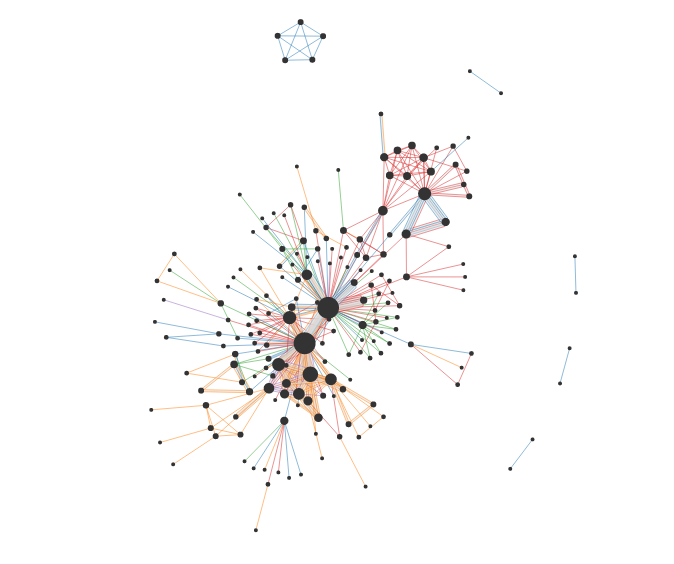
\includegraphics[trim={0 0 0 0}, width=140mm]{./Figures/marieBoucherFull.png}
  \caption{Marie Boucher network, full time period}
  \label{fig:marieBoucherFull}
  \end{center}
\end{figure}

-Only really one large component

-Some very central nodes

-Five satellite components

\begin{figure}[h!]
  \begin{center}
  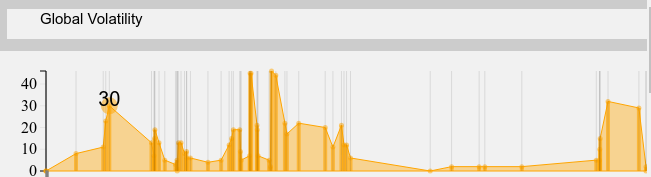
\includegraphics[trim={0 0 0 0}, width=140mm]{./Figures/marieBoucherGlobalVolatility.png}
  \caption{Marie Boucher Global Volatility}
  \label{fig:marieBoucherGlobalVolatility}
  \end{center}
\end{figure}

I'll begin by looking only at the global measures, starting with global volatility, Figure \ref{fig:marieBoucherGlobalVolatility}, we can see the network is initially erratic, then goes through very few changes for a sizeable portion of time, then has a burst of activity towards the end of the full period. 

\begin{figure}[h!]
  \begin{center}
  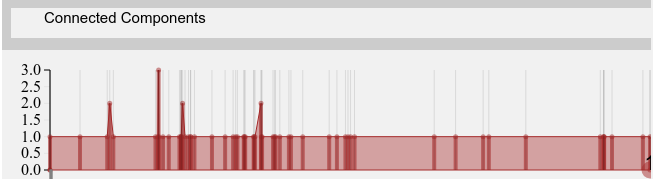
\includegraphics[trim={0 0 0 0}, width=140mm]{./Figures/marieBoucherConnectedComponents.png}
  \caption{Marie Boucher Connected Components}
  \label{fig:marieBoucherConnectedComponents}
  \end{center}
\end{figure}

Looking next at the number of connected components, Figure \ref{fig:marieBoucherConnectedComponents}, we find that for the majority of time frames there is only one connected component - there are three frames with two connected components and one frame with three connected components. Manually stepping through the graph we can also see that these components tend to be connected to one of two highly central nodes.

\begin{figure}[h!]
  \begin{center}
  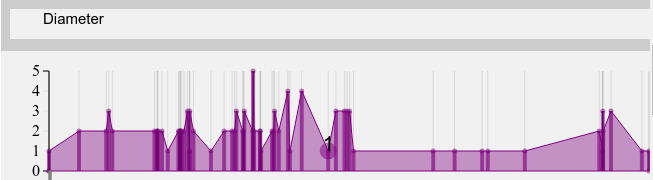
\includegraphics[trim={0 0 0 0}, width=140mm]{./Figures/marieBoucherDiameter.png}
  \caption{Marie Boucher Diameter}
  \label{fig:marieBoucherDiameter}
  \end{center}
\end{figure}

Looking next at Diameter, Figure \ref{fig:marieBoucherDiameter}, we see the same pattern we noticed in Global Volatility, erratic at first, a flat period of low activity then a jump at the end. There is a lot of variation in the values which could indicate that the network is quite different at each time frame. This is further enforced by density since it is similarly high in variation.

\begin{figure}[h!]
  \begin{center}
  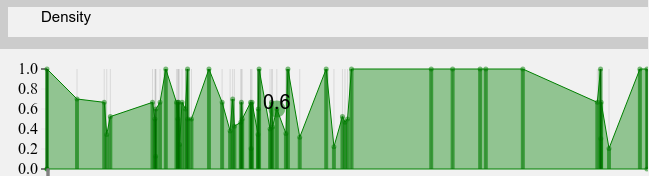
\includegraphics[trim={0 0 0 0}, width=140mm]{./Figures/marieBoucherDensity.png}
  \caption{Marie Boucher Density}
  \label{fig:marieBoucherDensity}
  \end{center}
\end{figure}

Density, Figure \ref{fig:marieBoucherDensity}, follows the same pattern. Interestingly, the density during the flat period is 100\%. Investigating this with the timeline slider we see that this is because there are only ever two nodes connected at a time during this period. 

\begin{figure}[H]
  \begin{center}
  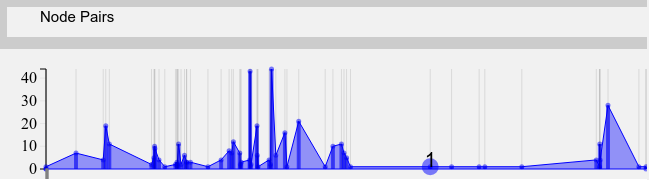
\includegraphics[trim={0 0 0 0}, width=140mm]{./Figures/marieBoucherNodePairs.png}
  \caption{Marie Boucher Node Pairs}
  \label{fig:marieBoucherNodePairs}
  \end{center}
\end{figure}

\begin{figure}[H]
  \begin{center}
  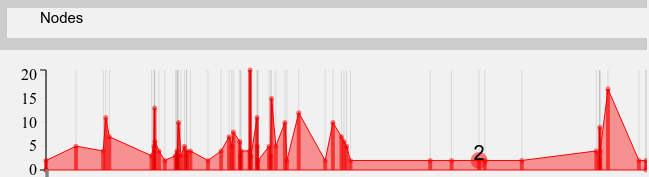
\includegraphics[trim={0 0 0 0}, width=140mm]{./Figures/marieBoucherNodes.png}
  \caption{Marie Boucher Nodes}
  \label{fig:marieBoucherNodes}
  \end{center}
\end{figure}

We could equally have confirmed this by looking at the number of node pairs, Figure \ref{fig:marieBoucherNodePairs}, and number of nodes, Figure \ref{fig:marieBoucherNodes}. The number of nodes is always 2 and number of nodepairs is always 1 during this flat period. The number of node pairs is very tightly correlated to the number of nodes here, the peaks could be worth further investigation as they are clearly periods of high activity relative to other frames.

\begin{figure}[h!]
  \begin{center}
  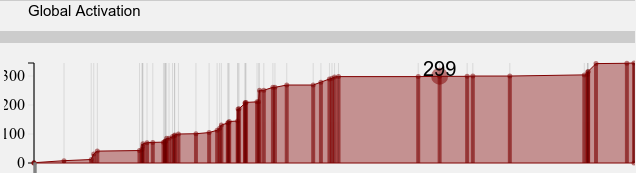
\includegraphics[trim={0 0 0 0}, width=140mm]{./Figures/marieBoucherGlobalActivation.png}
  \caption{Marie Boucher Global Activation}
  \label{fig:marieBoucherGlobalActivation}
  \end{center}
\end{figure}
Global activation, Figure \ref{fig:marieBoucherGlobalActivation}, increases reasonably linearly for the first period. Notably, during the flatter period it does increase slightly at each step confirming that the pairs we investigated in the density section are all different. 

\begin{figure}[H]
  \begin{center}
  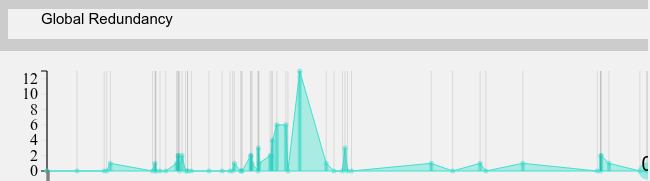
\includegraphics[trim={0 0 0 0}, width=140mm]{./Figures/marieBoucherGlobalRedundancy.png}
  \caption{Marie Boucher Global Redundancy}
  \label{fig:marieBoucherGlobalRedundancy}
  \end{center}
\end{figure}
Global redundancy, Figure \ref{fig:marieBoucherGlobalRedundancy}, is mostly fairly low, however there is one large peak which indicates further investigation could be useful as to why only that frame had many previously seen nodepairs, particularly as that specific frame wasn't identified as interesting by any of the other measures. The burst of activity at the end we noticed earlier isn't as obvious in this graph, indicating that most of the connections made in that period are new.
    
Looking more generally at the graphs, the spacing of the vertical lines also indicates three separate periods. We can also spot some periods and frames where many graphs have notable peaks or troughs that could spark further investigation.
    
\begin{center}
\begin{tabular}{cc}
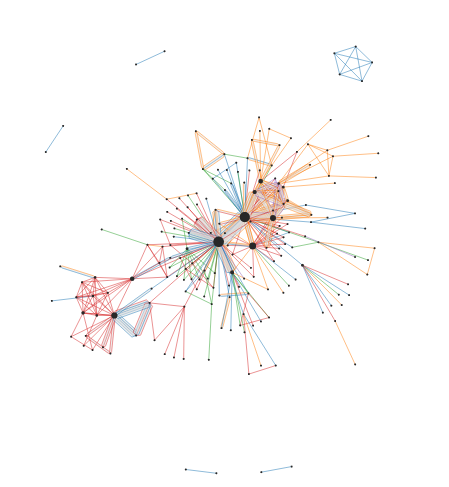
\includegraphics[trim={0 0 0 0}, width=140mm]{./Figures/marieBoucherLocalVolatilityFull.png}
\end{tabular}
\captionof{figure}{Marie Boucher - Local Volatility for the full time period}
\label{fig:marieBoucherLocalVolatilityFull}
\end{center}   
Next, the local measures can be investigated. Applying local volatility to the whole graph, Figure \ref{fig:marieBoucherLocalVolatilityFull}, we see that the two highly central nodes have high volatilities. This is because they make many fresh connections. Other fairly central nodes can be seen to have noticeably high volatilites. Standout nodes of interest here are more obvious than when the centrality measure is applied, as seen in Figure \ref{fig:marieBoucherLocalCentralityFull}.
\begin{center}
\begin{tabular}{cc}
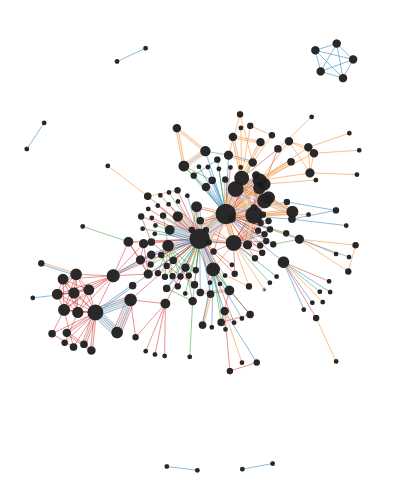
\includegraphics[trim={0 0 0 0}, width=85mm]{./Figures/marieBoucherLocalCentralityFull.png}
\end{tabular}
\captionof{figure}{Marie Boucher - Local Degree Centrality for the full period}
\label{fig:marieBoucherLocalCentralityFull}
\end{center}   


\begin{center}
\begin{tabular}{cc}
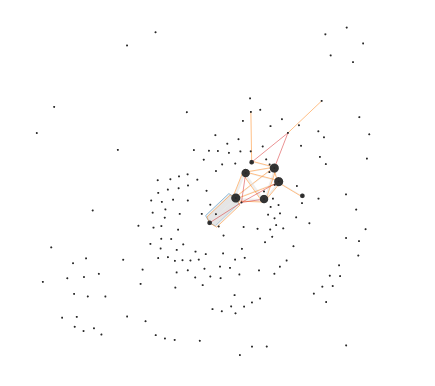
\includegraphics[trim={0 0 0 0}, width=85mm]{./Figures/marieBoucherLocalRedundancyPeriod1.png}
\end{tabular}
\captionof{figure}{Marie Boucher - Local Redundancy for a short period}
\label{fig:marieBoucherLocalRedundancyPeriod1}
\end{center}   
Applying local redundancy to the network, Figure \ref{fig:marieBoucherLocalRedundancyPeriod1}, and stepping through it, there are only a few nodes that particularly stand out as having high redundancy. As expected the central nodes tend to have higher values than the outer nodes but some of the tightly linked nodes have notable redundancies, showing that they are connected a few separate times in the full period.

\begin{center}
\begin{tabular}{cc}
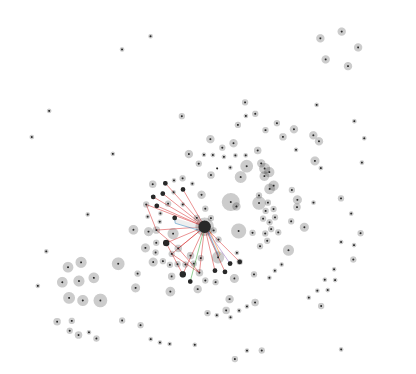
\includegraphics[trim={0 0 0 0}, width=140mm]{./Figures/marieBoucherLocalActivationPeriod1.png}
\end{tabular}
\captionof{figure}{Marie Boucher - Local Activation for a short period}
\label{fig:marieBoucherLocalActivationPeriod1}
\end{center} 
After switching to activation, Figure \ref{fig:marieBoucherLocalActivationPeriod1}, we can see many nodes score quite high as we step through the network, particularly the central nodes but also some of the outer nodes.

\section{Scenario 2 Turin Network}

[Reference and Summary]

The Turin network is much more seperated than Marie Boucher and much more cluster/component based. This makes it an excellent network to analyse alongside Marie Boucher.

\begin{center}
\begin{tabular}{cc}
\label{edgeTypes}
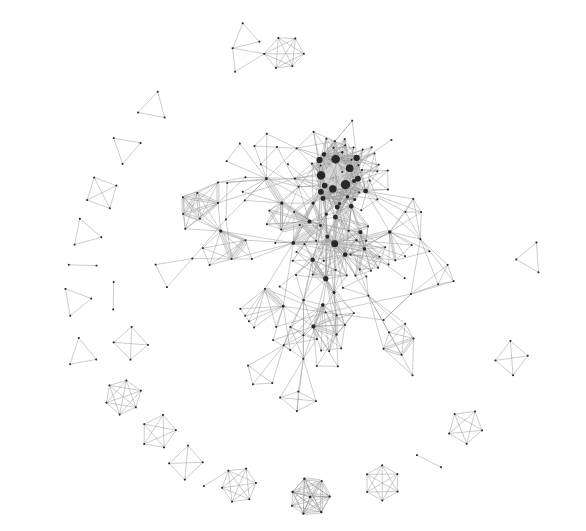
\includegraphics[trim={0 0 0 0}, width=140mm]{./Figures/TurinLocalVolatilityFull.png}
\end{tabular}
\captionof{figure}{The Turin Network, Local Volatility Measure Enabled}
\label{fig:TurinLocalVolatilityFull}
\end{center}

We begin again by looking at the global measures. Global volatility, Figure \ref{fig:TurinGlobalVolatility}, has around five periodic large jumps.

\begin{figure}[h!]
  \begin{center}
  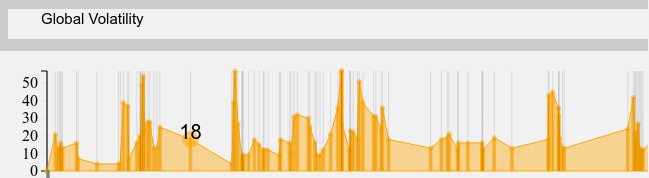
\includegraphics[trim={0 0 0 0}, width=140mm]{./Figures/TurinGlobalVolatility.png}
  \caption{Turin Global Volatility}
  \label{fig:TurinGlobalVolatility}
  \end{center}
\end{figure}

In between each of these jumps is reasonably high volatility, so together these indicate that there are occasional very large changes in the network and that in general the network is quite volatile and never really static for a period of time.
    
\begin{center}
\end{center}  

\begin{figure}[h!]
  \begin{center}
  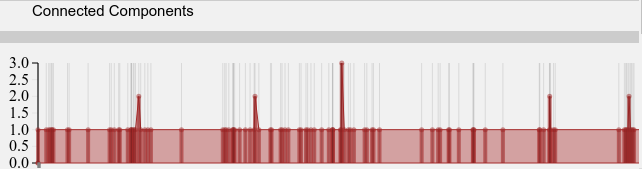
\includegraphics[trim={0 0 0 0}, width=140mm]{./Figures/TurinConnectedComponents.png}
  \caption{Turin Connected Components}
  \label{fig:TurinConnectedComponents}
  \end{center}
\end{figure}
Looking next at the number of connected components, Figure \ref{fig:TurinConnectedComponents}, if we observe the network itself and step through it then it is readily apparent that it is made of many small connected components which tend to become active for short periods. Interestingly, what this graph shows - combined with this observation about the network - is that for the majority of the time there is only one active connected component, with only four time frames occurring with two active and one time frame occurring with three active.

\begin{figure}[h!]
  \begin{center}
  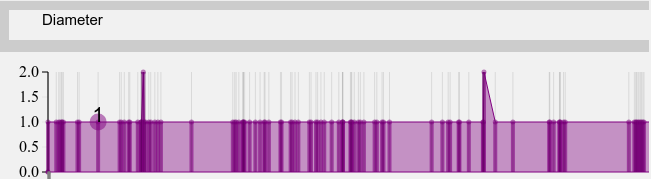
\includegraphics[trim={0 0 0 0}, width=140mm]{./Figures/TurinDiameter.png}
  \caption{Turin Diameter}
  \label{fig:TurinDiameter}
  \end{center}
\end{figure}
The diameter, shown in Figure \ref{fig:TurinDiameter}, is equally interesting, as there are only two time frames where the diameter is over one, and in both cases that value is two. Combined with what we know about connected components we can see that all of these components are highly connected since the vast majority only have a diameter of one, which is the smallest possible diameter for any network.
    
\begin{figure}[h!]
  \begin{center}
  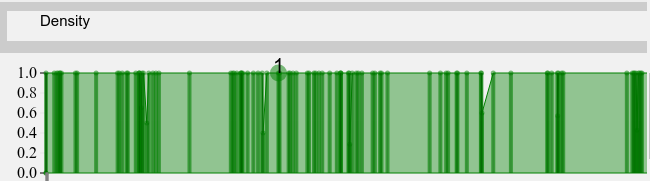
\includegraphics[trim={0 0 0 0}, width=140mm]{./Figures/TurinDensity.png}
  \caption{Turin Density}
  \label{fig:TurinDensity}
  \end{center}
\end{figure}
Adding density, Figure \ref{fig:TurinDensity}, further consolidates these findings as we can see that for the majority of time frames the components have a density of $1.0$. Combining this with what we've already discovered we now know that in most time frames we have a single connected component with every node in that component connected to every other node in that component. Two of the dips also align with the spikes in diameter.

\begin{figure}[h!]
  \begin{center}
  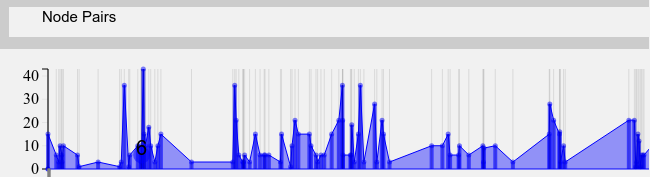
\includegraphics[trim={0 0 0 0}, width=140mm]{./Figures/TurinNodePairs.png}
  \caption{Turin Nodepairs}
  \label{fig:TurinNodePairs}
  \end{center}
\end{figure}

\begin{figure}[h!]
  \begin{center}
  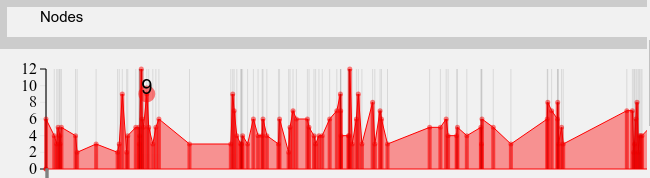
\includegraphics[trim={0 0 0 0}, width=140mm]{./Figures/TurinNodes.png}
  \caption{Turin Nodes}
  \label{fig:TurinNodes}
  \end{center}
\end{figure}
Due to the density and what we've observed previously, the number of nodepairs, Figure \ref{fig:TurinNodePairs}, and nodes, Figure \ref{fig:TurinNodes}, are naturally very tightly correlated. Comparing with the density graph we can see that the few blips in perfect correlation all match the fluctuations in density. Since we know this network tends to have one active fully connected component active in each time frame, we can now gain a sense of the sizes of each of these components. Comparing again with the connected components graph we can see that these large jumps tend to be linked with time frames where there is more than one connected component. Some of the blips in diameter and density also align with time frames with more than one connected component. The time frames these blips occur in could therefore be worth extra investigation.
    
\begin{figure}[h!]
  \begin{center}
  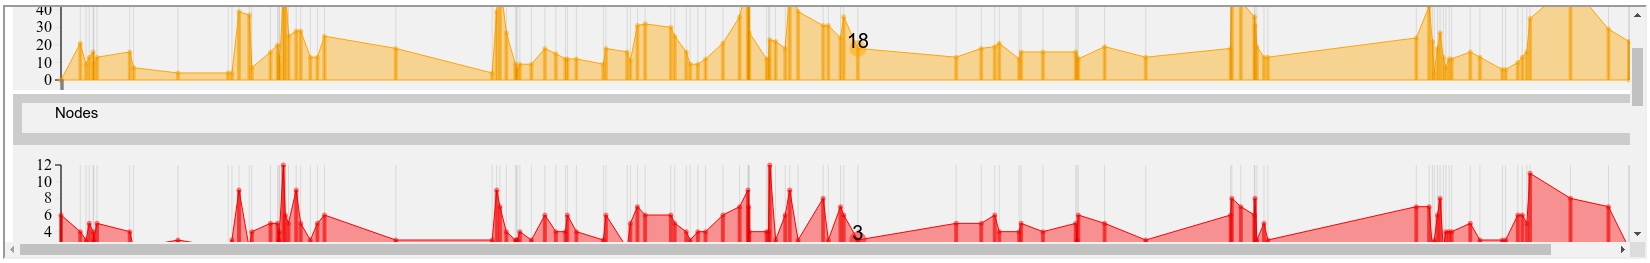
\includegraphics[trim={0 0 0 0}, width=140mm]{./Figures/TurinGlobalVolatilityAndNodes.png}
  \caption{Turin Global Volatility and Nodes comparison}
  \label{fig:TurinGlobalVolatilityAndNodes}
  \end{center}
\end{figure}

Comparing the number of nodes with Global Volatility, Figure \ref{fig:TurinGlobalVolatilityAndNodes}, by dragging the number of nodes graph up such that it is directly below the global volatility graph they can now be easily compared. We can see that the steps of very high volatility identified earlier are explained by the large new connected components appearing during those time frames.
   
\begin{figure}[h!]
  \begin{center}
  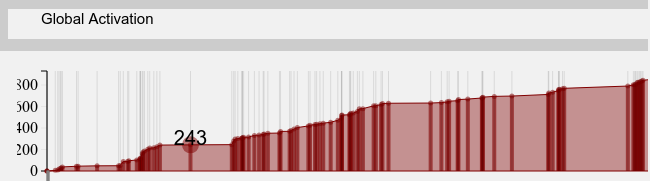
\includegraphics[trim={0 0 0 0}, width=140mm]{./Figures/TurinGlobalActivation.png}
  \caption{Turin Global Activation}
  \label{fig:TurinGlobalActivation}
  \end{center}
\end{figure}

Continuing down to Global Activation, Figure \ref{fig:TurinGlobalActivation}, we can see that new nodepairs are added at a fairly constant pace. Looking next at Global Redundancy, the peaks indicate that many of the nodepairs have been active before, we can use this alongside the network itself to easily find the components that appear more than once.

\begin{figure}[h!]
  \begin{center}
  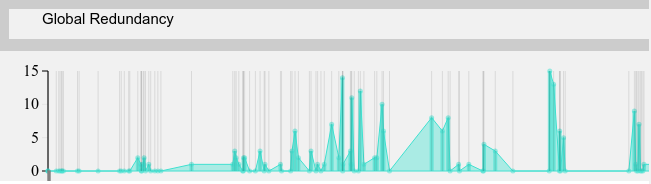
\includegraphics[trim={0 0 0 0}, width=140mm]{./Figures/TurinGlobalRedundancy.png}
  \caption{Turin Global Redundancy}
  \label{fig:TurinGlobalRedundancy}
  \end{center}
\end{figure}
Finally with Global Redundancy, Figure \ref{fig:TurinGlobalRedundancy}, the values appear highly erratic. This measure would be useful to see at which periods past business groups are reconnected. Dragging it to compare it with Global Volatility and Nodepairs we can see some correlation.


Looking more generally at all graphs we can gain some more insight. Looking at the spread of time frames by observing the vertical bars, we can identify periods of no change and periods of considerable change. 
    
\begin{center}
\end{center}

\begin{center}
\begin{tabular}{cc}
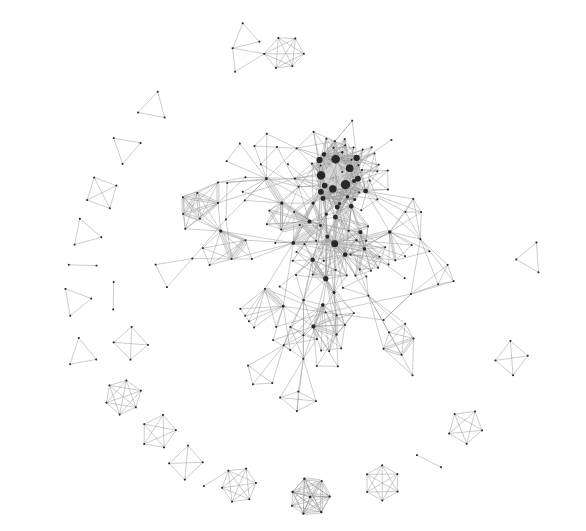
\includegraphics[trim={0 0 0 0}, width=140mm]{./Figures/TurinLocalVolatilityFull.png}
\end{tabular}
\captionof{figure}{Turin Local Volatility - Full time period}
\label{fig:TurinLocalVolatilityFull}
\end{center}
Next, we can experiment with the local measures. First with volatility, stepping through the network with a minimal window we see that the connected components tend to all have low similar volatilities with no standout nodes. Observing the full network over the whole time period we see that there is a large cluster containing several highly volatile nodes, Figure \ref{fig:TurinLocalVolatilityFull}. Stepping through the graph we see that this is because many of the connected components overlap in some way within this cluster of nodes. These nodes are therefore very worthy of further investigation as they are highly active and with many different nodes rather than a fixed number.


\begin{center}
\begin{tabular}{cc}
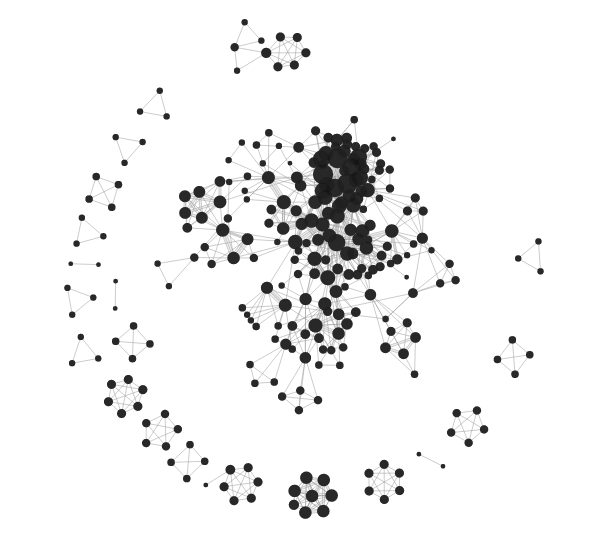
\includegraphics[trim={0 0 0 0}, width=140mm]{./Figures/TurinLocalCentralityFull.png}
\end{tabular}
\captionof{figure}{Turin Centrality - Full time period}
\label{fig:TurinLocalCentralityFull}
\end{center}

\begin{center}
\end{center}
Comparing these results from local volatility with the centrality measure - again applied to the whole graph, Figure \ref{fig:TurinLocalCentralityFull} - is interesting, because we can see that using local volatility makes the interesting nodes stand out much more. 
\begin{center}
\begin{tabular}{cc}
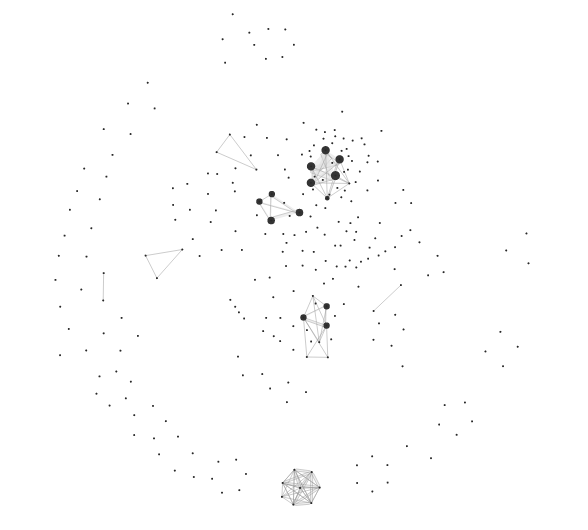
\includegraphics[trim={0 0 0 0}, width=140mm]{./Figures/TurinLocalRedundancy1.png}
\end{tabular}
\captionof{figure}{Turin Local Redundancy - short time period}
\label{fig:TurinLocalRedundancy1}
\end{center}
Switching to local redundancy and selecting a period towards the end of the network's timeline, Figure \ref{fig:TurinLocalRedundancy1}, we can easily spot the components that have been active at some point before that period as they have a redundancy greater than zero. This further complements our findings from the global redundancy measure.

\begin{center}
\begin{tabular}{cc}
\label{edgeTypes}
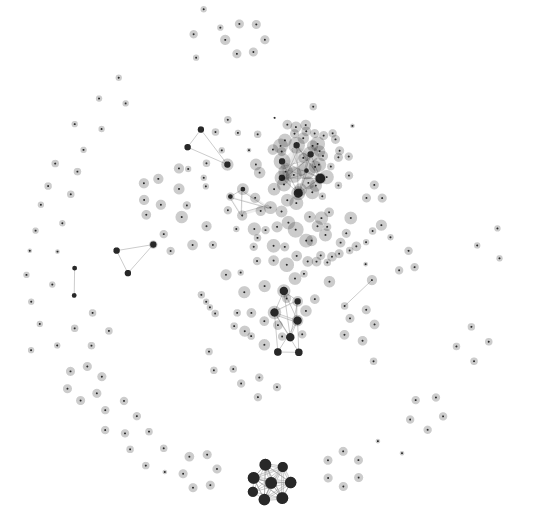
\includegraphics[trim={0 0 0 0}, width=140mm]{./Figures/TurinLocalActivation.png}
\end{tabular}
\captionof{figure}{Turin Local Activation - same short time period}
\label{fig:TurinLocalActivation}
\end{center}
Switching directly to local activation from here, Figure \ref{fig:TurinLocalActivation}, and looking again at the components identified as having higher redundancy we can see how high the activation in the selected time period is relative to the total network activity by comparing with the grey outer circles. Since they aren't considerably larger for any node in these components we could infer that this component is likely only fully active one or two times before this period.

\section{Scenario 3 - Marguerite} 

\begin{multicols}{2}
\begin{center}
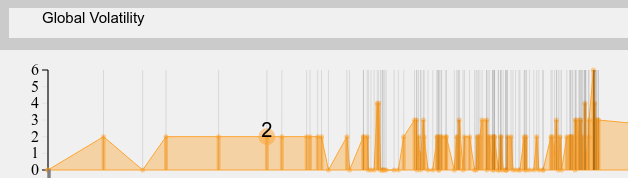
\includegraphics[trim={0 0 0 0}, width=60mm]{./Figures/margueriteGlobalVolatility.png}
\end{center}
\begin{center}
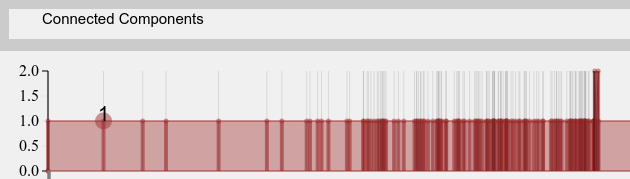
\includegraphics[trim={0 0 0 0}, width=60mm]{./Figures/margueriteConnectedComponents.png}
\end{center}
\begin{center}
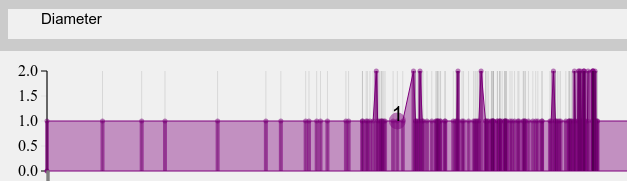
\includegraphics[trim={0 0 0 0}, width=60mm]{./Figures/margueriteDiameter.png}
\end{center}
\begin{center}
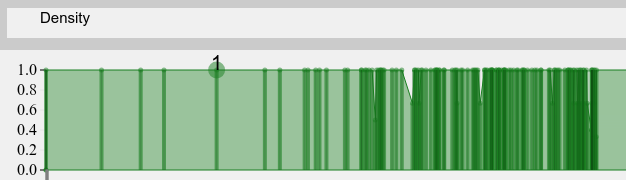
\includegraphics[trim={0 0 0 0}, width=60mm]{./Figures/margueriteDensity.png}
\end{center}
\begin{center}
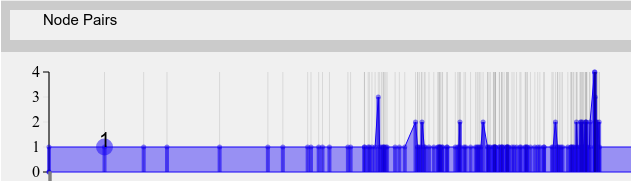
\includegraphics[trim={0 0 0 0}, width=60mm]{./Figures/margueriteNodePairs.png}
\end{center}
\begin{center}
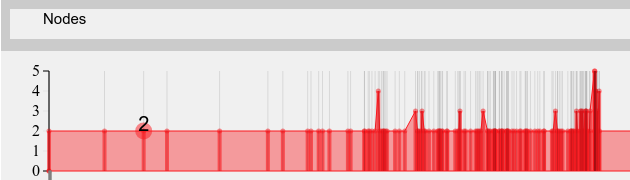
\includegraphics[trim={0 0 0 0}, width=60mm]{./Figures/margueriteNodes.png}
\end{center}
\begin{center}
\includegraphics[trim={0 0 0 0}, width=60mm]{./Figures/margueriteGlobalActivation.png}
\end{center}
\begin{center}
\includegraphics[trim={0 0 0 0}, width=60mm]{./Figures/margueriteGlobalRedundancy.png}
\end{center}
\captionof{figure}{All Global Measures for Marguerite Network}
\label{fig:margueriteAllGraphs}
\columnbreak
[Reference]
Finally, to assess the power of the measure based approach, we could try looking solely at the global measures of a new network to see how much information we can gleam, Figure \ref{fig:margueriteAllGraphs}. 

Looking generally at all graphs we can see there is fairly little activity in the first half and then a lot in the second. We can see that for most time frames there are only two nodes involved - explaining the density and diameter - and steadily increasing global activation implying that many new nodes are connected to. What's very interesting however is that global redundancy for the second half tends to be one. Tying this together and the picture we get is either of a network primarily composed of one node connecting to many new nodes in the second period or many pairs becoming active where one of the nodes in the pair has been active before. Looking more closely at the values of global activation which appear to increase by one during each time frame in this period and we can rule out the second option.
\end{multicols}

Looking at the actual network, Figure \ref{fig:margueriteNetwork}, these findings were accurate. 

\begin{figure}[h!]
  \begin{center}
  \includegraphics[trim={0 0 0 0}, width=40mm]{./Figures/margueriteNetwork.png}
  \caption{Marguerite Full Network}
  \label{fig:margueriteNetwork}
  \end{center}
\end{figure}
[Summary and reference for the Marguerite network.]
Of course, the measures are meant to be complementary to the network and not to replace it, but being able to extract this much information solely from them with relative ease indicates that they are a powerful tool.

\pagebreak
\section{Directly comparing Marie Boucher and Turin}
\begin{multicols}{2}
\begin{center}
\includegraphics[trim={0 0 0 0}, width=60mm]{./Figures/marieBoucherGlobalVolatility.png}
\end{center}
\begin{center}
\includegraphics[trim={0 0 0 0}, width=60mm]{./Figures/marieBoucherConnectedComponents.png}
\end{center}
\begin{center}
\includegraphics[trim={0 0 0 0}, width=60mm]{./Figures/marieBoucherDiameter.png}
\end{center}
\begin{center}
\includegraphics[trim={0 0 0 0}, width=60mm]{./Figures/marieBoucherDensity.png}
\end{center}
\begin{center}
\includegraphics[trim={0 0 0 0}, width=60mm]{./Figures/marieBoucherNodePairs.png}
\end{center}
\begin{center}
\includegraphics[trim={0 0 0 0}, width=60mm]{./Figures/marieBoucherNodes.png}
\end{center}
\begin{center}
\includegraphics[trim={0 0 0 0}, width=60mm]{./Figures/marieBoucherGlobalActivation.png}
\end{center}
\begin{center}
\includegraphics[trim={0 0 0 0}, width=60mm]{./Figures/marieBoucherGlobalRedundancy.png}
\end{center}
\captionof{figure}{Marie Boucher Network}
\label{fig:marieBoucherAllGraphs}
\columnbreak



\begin{center}
\includegraphics[trim={0 0 0 0}, width=60mm]{./Figures/TurinGlobalVolatility.png}
\end{center}
\begin{center}
\includegraphics[trim={0 0 0 0}, width=60mm]{./Figures/TurinConnectedComponents.png}
\end{center}
\begin{center}
\includegraphics[trim={0 0 0 0}, width=60mm]{./Figures/TurinDiameter.png}
\end{center}
\begin{center}
\includegraphics[trim={0 0 0 0}, width=60mm]{./Figures/TurinDensity.png}
\end{center}
\begin{center}
\includegraphics[trim={0 0 0 0}, width=60mm]{./Figures/TurinNodePairs.png}
\end{center}
\begin{center}
\includegraphics[trim={0 0 0 0}, width=60mm]{./Figures/TurinNodes.png}
\end{center}
\begin{center}
\includegraphics[trim={0 0 0 0}, width=60mm]{./Figures/TurinGlobalActivation.png}
\end{center}
\begin{center}
\includegraphics[trim={0 0 0 0}, width=60mm]{./Figures/TurinGlobalRedundancy.png}
\end{center}
\captionof{figure}{Turin Network}
\label{fig:turinAllGraphs}
\end{multicols}

Interestingly, when looking at the actual networks themselves, Figure \ref{fig:TurinLocalVolatilityFull} and Figure \ref{fig:marieBoucherFull}, despite the fact that they appear to be quite different, the global measure graphs, Figures \ref{fig:marieBoucherAllGraphs} and \ref{fig:turinAllGraphs}, seem moderately similar at a glance. This is likely because whilst actually stepping through each time frame, the networks behave similarly in that there are usually only a few nodes involved and they tend to be in a single component. The difference, which can be seen in the diameter and density graphs, is that in the Marie Boucher network these components tend to be made up of one central node with the other active nodes mostly only connected to it, but in the Turin network, the nodes tend to be more interconnected.


\chapter{Discussion}

In this paper I have presented a measure based approach to dynamic network visualisation. Details of the measures and their implemented visualisation have been provided.

\section{Potential further work} 
Creating visualisations is a highly iterative and experimental process, so naturally many ideas have been produced for improvements that could be made to the system. This section details some of those potential improvements.
\newline

Automatically highlighting points of interest could be a useful feature, by looking at the "interestingness" of each timeframe. These points of interest would be timeframes where many of the global measures differ significantly from their average and could be considered outliers. The most significant, say, three of these timeframes could then be shown on the timeline. One possible way to achieve this that I considered would be using Tukey fences, which can be used to spot outliers. David C. Hoaglin in John W. Tukey and Data Analysis \cite{jwtada} states that Exploratory Data Analysis \cite{eda} uses "fences" to flag possible outliers. These are based on the "hinges," $H_L$ and $H_U$, which are approximate quartiles of the batch. He goes on to say that the basic idea is to calculate the H-spread, $d_H = H_U - H_L$, and lay off a multiple of it below $H_L$ and above $H_U$: 
\begin{equation}
 H_L-kd_H \, \, and \, \, H_U + kd_H.
\end{equation}
He continues to say that the limited preliminary edition (Tukey, 1970c) used k = 1.0 for the "side values" and k = 1.5 for the "three-halves values." By the first edition (Tukey, 1977a) the constants had changed a lot, to k = 1.5 for the "inner fences" and k = 3.0 for the "outer fences," with the labels "outside" and "far out," respectively, for data values beyond them.
Finally he states that the aim was not to have a formal rule for declaring an observation an outlier, but to call attention to such data for further investigation. The values of k have remained at 1.5 and 3.0, and the "inner fences" naturally see more use in practice. 
Since the goal is not to formally rule on outliers but rather to "call attention to such data for further investigation", this method could work well for calculating a sense of 'interestingness'.
\newline

Adding more measures is an obvious improvement - particularly local dynamic measures as they aren't found in other tools. An example could be a measure to add a sense of node 'promiscuity' - if volatility focuses on how the lifespans of node-pairs vary over time then 'promiscuity' would focus more on how often those edges tend to be with the same nodes. A node that had a few fairly rigid connections but also made a new connection every time step would have relatively low volatility but high promiscuity. A node that erratically gained and lost connections but only to a select few nodes would have high volatility but low promiscuity.
\newline

The grey node 'halos' shown in Figure \ref{fig:greyCircles} could be adjusted such that instead of being fixed to the full time period, the could be locked to the currently selected period with a button. This would allow a user to select one period, lock that selection so that the 'halos' are recalculated, then change their time period selection and compare the new node sizes with the "halo" sizes for a given local measure.
\newline

Adding the ability to move the databar into a separate window, which could then be dragged to a separate screen - creating more space for the node-link diagram and allowing more graphs in the databar to be visualised at once. 
\newline

Running a think-aloud study or similar user trial could be useful to discover more about how effective the current implementation is and provide insight into further improvements.
\newline

Another improvement mentioned during the feedback meeting (and briefly considered before) was enabling graphs to be exported as a png to allow for easy insertion into academic papers. This would encourage adoption and improve quality of life for end users.
\newline


\section{Evaluation of work completed} 
The number of connected components measure could perhaps be replaced with a cluster based measure, which would likely achieve a similar effect while also capturing the clusters. The basic global measures - number of nodepairs and number of nodes - tend to overlap in terms of information provided since they're highly correlated. However having one without the other seems somewhat incomplete. Density and Diameter both provide useful information and I found them to be good indicators of the network structure. Global activation, redundancy and volatility were the more experimental and dynamic measures. I found that the three of them have a strong synergy when observed together since they're specifically dynamic. Perhaps more global dynamic measures could be added but I don't think any of those three should be removed. Local measures are slightly more situational, volatility works well in showing specifically interesting nodes. Activation and redundancy again work well for highlighting new or old relationships. I believe there is certainly scope for more local measures, particularly dynamic measures.

If this project were to be continued further, I would recommend first attempting to source some feedback on the existing implementation to better guide any further changes. I feel that enough measures have been implemented, and that the user interface is intuitive enough to properly demonstrate the measure based approach, providing better feedback. I would recommend getting familiar with the codebase, particularly understanding how the iframes interact with each other. Both the local and global measure implementations are readily extensible, I've found that many measures share data structures and methods making new measures even easier to implement.
I would also recommend bearing scalability in mind when adding any new measures. Working within the browser is limiting, so data structures and algorithms need to be well thought out to run smoothly - particularly for local measures as they are constantly recalculated as the time period is adjusted.

The meeting with network scientists validated the approach and the system works well in the described usage scenarios. I'm confident that a measure based approach works well as a dynamic network visualisation when used alongside a nodelink diagram. More specifically, most measures appear to be useful in their own right although there can be occasional overlap in the information they provide. 


\appendix
%%%%%%%%%%%%%%%%%%%%%%%%%%%%%%%%%%%%%%%%%%%%%%%%%%%%%%%%%%%%%%%%%%%%%%%%%%%%%%%%%
%2345678901234567890123456789012345678901234567890123456789012345678901234567890
%        1         2         3         4         5         6         7         8
% THESIS APPENDIX

\chapter{Gesture Vocabulary} 
\label{chap:appendixA}


\begin{figure}
    \centering
    \includegraphics[width=0.8\textwidth]{Chapter4/Figures/Figures/gv.PNG}
    \caption{Proposed gesture vocabulary}
    \label{fig:gs}
\end{figure}


%\chapter{Survey}
\label{chap:appendixB}


%\begin{figure}
%\setboolean{@twoside}{false}
% Uncomment the follow line to show the survey
\includepdf[pages=1-,scale=0.8,pagecommand={}]{Appendix2/gbhri3_format.pdf}
%\end{figure}

%\begin{figure}
 %\centering 
 %\includegraphics{Appendix2/gbhri3_format.pdf}
%\end{figure}
%\bibliographystyle{Classes/RoboticsBiblio}    % bibliography style
\bibliographystyle{ieeetr}
\renewcommand{\bibname}{References}           % change default name Bibliography to References
%\addcontentsline{toc}{section}{References}
\nocite{*}
\begin{appendices}
\chapter{Local Volatility Examples}

While the results are intuitive, the specifics of how local volatility is calculated are slightly complex, so some additional examples are provided in this appendix.

\label{appendix:appendixA}
In this network, a nodepair exists between the central node, A, and each of the four surrounding nodes for one frame each. The volatility values for nodes A and B are calculated. All nodes other than A will have the same value as B. We can observe that the local volatility of A is considerably higher than B, as would be expected.
\begin{center}
\includegraphics[trim={0 15cm 0 0}, width=140mm]{./Figures/volatilityAppendix1.png}
$local\ volatility(A) = std([1,0,0,0]) + std([0,0,0,1]) + std([0,1,0,0]) + std([0,0,1,0])$

$local\ volatility(A) = 1.73$

$local\ volatility(B) = std([1,0,0,0])$

$local\ volatility(B) = 0.43$
\end{center}

In this network, nodepair 1 is active between node A and node B for three time frames, in the fourth timeframe nodepair 2 is active instead. The volatility values for nodes A and B are calculated. We can observe that the local volatility of A is higher than B, as would be expected, but lower than the previous example. This again is intuitive because A makes fewer connections than the previous example.
\begin{center}
\includegraphics[trim={0 15cm 0 0}, width=140mm]{./Figures/volatilityAppendix2.png}
$local\ volatility = std([1,1,1,0]) + std([0,0,0,1])$

$local\ volatility(A) = 0.86$

$local\ volatility(B) = std([1,1,1,0])$

$local\ volatility(B) = 0.43$
\end{center}

In this network node A always has two active nodepairs, these vary in each timeframe. The volatility values for nodes A and B are calculated. We can observe that the local volatility of A is much higher than B, as would be expected, and even higher than the first example. This again is intuitive because A makes many more connections with all of them appearing twice. B is slightly higher because it's nodepair is active twice.
\begin{center}
\includegraphics[trim={0 15cm 0 0}, width=140mm]{./Figures/volatilityAppendix3.png}
$local\ volatility = std([1,0,1,0]) + std([0,1,1,1]) + std([1,0,0,1]) + std([0,1,0,1])$

$local\ volatility(A) = 2$

$local\ volatility(B) = std([1,0,1,0])$

$local\ volatility(B) = 0.5$
\end{center}

In this network all edges are fixed for the full time period with no changes, so the volatilities for node A and B are both, as expected, 0.
\begin{center}
\includegraphics[trim={0 15cm 0 0}, width=140mm]{./Figures/volatilityAppendix4.png}
$local\ volatility = std([1,1,1,1]) + std([1,1,1,1]) + std([1,1,1,1]) + std([1,1,1,1])$

$local\ volatility(A) = 0$

$local\ volatility = std([1,1,1,1])$

$local\ volatility(B) = 0$
\end{center}

%\chapter{Local Activation and Redundancy Examples}
%\begin{center}
%\includegraphics[trim={0 15cm 0 0}, width=140mm]{./Figures/volatilityAppendix1.png}
%$local\ activation(A) =$

%$local\ redundancy(A) =$

%\end{center}
%\begin{center}
%\includegraphics[trim={0 15cm 0 0}, width=140mm]{./Figures/volatilityAppendix2.png}
%$local\ activation(A) =$

%$local\ redundancy(A) =$
%\end{center}
%\begin{center}
%\includegraphics[trim={0 15cm 0 0}, width=140mm]{./Figures/volatilityAppendix3.png}
%$local\ activation(A) =$

%$local\ redundancy(A) =$
%\end{center}
%\begin{center}
%\includegraphics[trim={0 15cm 0 0}, width=140mm]{./Figures/volatilityAppendix4.png}
%$local\ activation(A) =$

%$local\ redundancy(A) =$
%\end{center}

\end{appendices}

\bibliography{References/references}          % References file
\addcontentsline{toc}{chapter}{References}    % add References to contents page

\end{document}
